\documentclass[12pt, letterpaper]{article}
\usepackage{graphicx}
\usepackage{textcomp}
\usepackage{geometry}
\usepackage{hyperref}
\usepackage{parskip}
\usepackage{setspace}
\usepackage{url}
\usepackage{cite}
\usepackage{float}
\usepackage{algorithm}
\usepackage{algpseudocode}
\usepackage{array}
\usepackage{svg}
\usepackage{svg-extract}
\usepackage{pdfpages}
\usepackage{subcaption}


\graphicspath{{./images/}}
\svgpath{{./images_svg/}}
\svgsetup{  inkscapeexe="C:/Program Files/Inkscape/bin/inkscape.exe"}

\renewcommand{\listfigurename}{List of Figures}
\renewcommand{\appendix}{Appendix}


\title{CREATING TACTILE PHOTOS THAT PEOPLE WITH VISUAL IMPAIRMENTS CAN ENJOY USING GENERATIVE AI AND 3D PRINTERS}

\author{S.PHABMIXAY Le-Tien-Vinh}
\date{August 2024}


\begin{document}
\maketitle

\begin{center}

    \vspace{2cm}
    \underline{Supervisor      Associate Professor Masakazu Iwamura}
    \vspace{4cm}
    
    A MASTER THESIS
    \vspace{1cm}
    
    Presented to the Department of Core Informatics,
    
    the Graduate School of Informatics of Osaka Metropolitan University
    
    for the degree of
    
    Master of Informatics
    
\end{center}


\newpage 

\vspace*{\fill}
\begin{center}
    \textcopyright S.PHABMIXAY Le-Tien-Vinh
\end{center}
\vspace*{\fill}

\newpage

\begin{center}
    ACKNOWLEDGMENTS
\end{center}
\vspace{1cm}
\paragraph{}
I extend my heartfelt gratitude to my esteemed professor, Dr. Masakazu Iwamura, whose unwavering guidance and support have been instrumental in shaping my journey throughout
my master’s program. Their exceptional expertise and encouragement motivated me to overcome challenges and complete this research, culminating in the writing of this thesis.
\paragraph{}
I am sincerely thankful to Dr. Koichi Kise, Osaka Metropolitan University, and ENSEA for providing me with the invaluable opportunity to conduct my research at
Osaka Metropolitan University and for generously offering the necessary resources and unwavering support throughout this endeavor.
\paragraph{}
I cannot overlook the immense support and love from my family, and friends I have met during my stay in Japan who
stood by my side during this enriching process. Their constant support and belief in my abilities have pushed me towards the completion of the writing of this master's thesis.
\paragraph{}
I would also like to sincerely thank Banri Kakehi and Yoh Otsuka, for their invaluable help not only with my integration to the laboratory but also with any problem I had encountered while
conducting this research, as well as the members of the Intelligent Media Processing laboratory for their comments and encouragements.
Their support was essential to the successful completion of this research.

\newpage




\tableofcontents{}
\newpage


\begin{spacing}{1.15}

\listoffigures
\listoftables
\addcontentsline{toc}{section}{\listfigurename}

\newpage

%%%%%%%%%%%%%%%%%%%% INTRODUCTION %%%%%%%%%%%%%%%%%%%%%%%%
\section{Introduction}

\paragraph{}
In an increasingly visually driven world, individuals with visual impairments often encounter significant barriers in accessing
visual information. Traditional means of communication and artistic expression, such as photographs and visual artwork, are predominantly
designed for sighted individuals, leaving those with visual impairments at a disadvantage. According to the World Health Organisation \hyperlink{WHOtarget}{[WHO]}. %Insert reference, 
more than 2.2 billion people live some kind of visual impairment, making them struggle in their daily life activities. This number can seem
excessive, but in reality, these visual impairments include not only blind people but also people with less
severe or renowned conditions. Non exhaustively, these include partial or full vision loss, or visual acuity \hyperlink{NMtarget}{[NM]}. %Insert reference
This discrepancy underscores a critical need for innovative solutions that can bridge the sensory divide and offer meaningful and engaging
experiences to all individuals, regardless of their visual capabilities.
\paragraph{}
The smartphone has widely become an essential tool over the past decade. With its initial design, the smartphone was undeniably made for
people without visual impairment, with the screen covering more than 90\% of its main face. Even so, the tactile property of the screen makes it
a useful tool in assisting people with visual impairments, along with its integrated speaker. In this context, current smartphone applications aim
to guide and assist people with visual impairments, and some of them have paved the way to more inclusive smartphone usage and the spread of more
comprehensive accessibility tools, such as ``Seeing AI \hyperlink{SeeAItarget}{[SeeAI]}" %Insert reference
which is an assistive application that provides an audio description of the user's surrounding objects by analyzing them after taking a photo.
Some other researches aim to help people with visual impairments be safe, for example by detecting fire in their habitation \hyperlink{MBC22target}{[MBC22]}. %Insert reference
This research relies not only on smartphones but also on security cameras to detect hazardous fire or ignition.
\paragraph{}
Recent advancements in technology, particularly in the fields of artificial intelligence (AI) and 3D printing, present new opportunities to
address this ``sensory gap", which is the unbalanced access to information due to sensory differences which is vision in this case.
 Generative AI, which leverages complex algorithms to create content based on input data, and 3D printing, which allows for
the creation of tangible objects from digital models, offer promising avenues for developing accessible and immersive experiences for people
with visual impairments.
\paragraph{}
Current methods for conveying visual information to individuals with visual impairments are often limited in scope and effectiveness as well as accessibilty.
Traditional tactile representations, such as raised-line drawings or dot-diagrams, do not fully capture the richness and detail of visual content. Other methods
such as full 3D printing is either time consuming or requires the expertise of a knowledgeable person, which does not render the process autonomous.
Furthermore, the creation of these tactile images is typically labor-intensive and may lack the depth and nuance that could enhance the
tactile experience.
\paragraph{}
This thesis explores the potential of integrating generative AI and 3D printing technologies to create tactile photos that can offer a more
nuanced and engaging experience for individuals with visual impairments. By leveraging AI's ability to analyze and interpret visual data and
3D printing's capability to produce detailed and customized tactile models, this research aims to develop a novel approach to creating tactile
photos that are both accessible and enjoyable.
The significance of this study lies in its potential to revolutionize the way visual information is presented to individuals with visual
impairments. By combining generative AI and 3D printing, this research aims to offer a more immersive and detailed tactile experience,
enriching the accessibility and enjoyment of visual content. This could lead to broader implications for \emph{educational materials}, artistic
expression, and everyday information, ultimately fostering a more inclusive and equitable society.
\paragraph{}
This thesis proposes a pipeline in which the user inputs a photo which is in the end printed using a 3D printer. A few points need to be followed for
it to be complete:
\begin{enumerate}
    \item Be an automated process and easy to use so that a person with visual impairment can use right away without any prior knowledge
    \item Be suited for educational purposes
\end{enumerate}
The second point here mainly involves printing the object in dimensions suitable for teaching. Traditional educational materials are given in A4
format. For storage purposes, we have also thought making the printed objects' thickness 5 centimeters at most. Ultimately, a durable plastic material
is to be used to ensure robustness of the object.
\paragraph{}
Most current 3D reconstruction methods involve reconstructing the object entirely by teaching the generative AI model priors, to ``guess" the shape of
the unseen part of the object. Following the constraints mentioned above, this is not what we are aiming at.
Instead we want only to print the visible part of the object, and give it depth and topography, so that people with visual impairment can understand
what the composition of the printed object is, understand the shapes of the contained object by touching and feeling it.
To complete such task, our method proposes a novel method that involves the usage of depth maps. Indeed, the method uses state-of-the-art depth estimation
networks that can generate accurate depth maps from an input 2D image. The depth map generated is then converted into detailed 3D models suitable
for tactile printing.
\paragraph{}
This study mainly focuses on the following points : explore the current state of technology in generative AI and 3D printing as they relate to
the creation of tactile content, design and implement a method for generating tactile photos using AI and 3D printing that accurately reflects
the depth and detail of the original visual content, and finally to assess the effectiveness and usability of the generated tactile photos through
user testing and feedback from individuals with visual impairments.
\paragraph{}
In summary, this research aims to provide insights on how people with visual impairments can interpret and perceive objects at a reduced scale, as they
are in a photo, which people without visual impairment can distinguish and recognize as they contain cues that we have learned prior to looking at the
said photo. While the method could not be tested on users, it is interesting to try to understand how people with visual impairment would translate
knowledge they have learned by touch to a different scale.

\newpage


%%%%%%%%%%%%%%%%%%%% Literature review %%%%%%%%%%%%%%%%%%%%%%%%

\section{Literature review}
\paragraph{}
In this chapter, we will oversee some existing research and applications that showcase what methods have led to what is currently available in assisting people with
visual impairment, and the current state generative AI that can be applied to the task of 3D modeling. It will explore the existing body of work
across the following key domains: tactile graphics, generative AI for image interpretation and 3D printing for accessibility. The literature review
aims to contextualize the development of tactile photos within these fields and identify the technological advancements and challenges associated with this endeavor.

\subsection{Tactile graphics for visual impairments}
\paragraph{}
For a long time, tactile graphics have been used to convey visual information to individuals who are blind or have low vision. Traditional methods involve
creating raised-line drawings, texture, symbols or embossed images that can be felt and interpreted by touch, for instance Braille being the most prominent reading method for
individuals who are blind or have diminished vision capabilites. Early research by Kennedy (1993) \hyperlink{Ken93target}{[Ken93]} highlights the
importance of simplifying visual content to be suitable for tactile interpretation, emphasizing the need for clear, unambiguous lines and shapes. Seiichi Miyake, in a quest
to help individuals with visual impairments navigate in the streets, first introduced \emph{tactile paving} in 1967 in the city of Okayama. The striped pavings would indicate
the user that they are on as sidewalk and should move forward, while dotted pavings indicate them to stop, at a crossing for instance. Jiangyan Lu et al. \hyperlink{LWXtarget}{[LWX08]}
have compared the different tactile paving design standards across several countries. Focusing on the factors of type, form and colour in constituting the standards of tactile paving,
this paper tries to identify the problems of tactile paving in China, and then gives some suggestions and insights for consideration and further investigation.


\paragraph{}
Some old studies have shown that tactile graphics can significantly enhance the learning and comprehension abilities of visually impaired individuals, and thus for
a long time (Edman in 1992). Tactile graphics are used in various fields, including education, navigation, and art appreciation. The primary challenge in creating tactile graphics
is ensuring that they are both detailed enough to convey necessary information and simple enough to be easily interpreted through touch (Heller in 2000 \hyperlink{Hel00target}{[Hel00]}).
Continuously, some have focused on enhancing the complexity and depth of tactile graphics. Lahav \& Mioduser (2008) \hyperlink{LM08target}{[LM08]} explored the use of tactile
maps for navigation, demonstrating how tactile graphics can be effectively used to communicate spatial information. However, traditional methods often fall short in conveying
detailed and nuanced visual content, such as photographs, which limits their applicability in certain contexts.


As mentioned previously, though Braille is common in areas where the user requires information, for instance an elevator where the user must read the buttons to know which floor to
go up to, or in the city when touching a map to find their direction, the Braille method shows its limitation in terms of range. As an individual without severe visual impairment such
as blindness or low vision can understand their surroundings and scenes very far from them thanks to their vision, it is difficult for a visually impaired individual to understand
the environment other than what is very close to them.

\subsection{Generative AI for image interpretation and depth Estimation}
\paragraph{}
The advent of generative AI has significantly expanded the possibilities for creating tactile graphics. AI algorithms, particularly those based on deep learning, have shown
remarkable capabilities in interpreting and generating images. Goodfellow et al. (2014) \hyperlink{GPM14target}{[GPM14]} introduced Generative Adversarial Networks (GANs), which have become a foundational
tool in generating realistic images from various input data. Variational Autoencoders have also shown remarkable capabilites in interpreting and generating images. Complex patterns can
be learnt by these models and they can generate new images with the learned characteristics.

In the context of visual impairments, researchers have explored the use of AI to create more meaningful and accessible content. Geirhos et al. (2018) \hyperlink{GMR18target}{[GRM18]}discussed the robustness of
deep learning models in image recognition and generation, highlighting their potential for accessibility applications. They have provided evidence that recognition models rely on
textures rather than shapes which is counterintuitive per say. They aim to move towards more realistic models of human visual object recognition.

\paragraph{}
Depth estimation, which can be deemed a critical component in generating tactile models from images, has also seen significant progress. However it has been a challenging issue in
computer vision. Early models use Convolutional Neural Networks to extract features from image and predict depth values for each pixel.\hyperlink{EPF14target}{[EPF14]} Ranftl et al. (2020) \hyperlink{RLH20target}{[RLH20]}
developed MiDaS, a state-of-the-art monocular depth estimation model that generates detailed depth maps from 2D images. This work states that the massive amount of datasets are the 
cause of the success of deep networks, but they are still insufficient for monocular depth estimation (meaning depth estimation from a single image). It proposes a generalization
method to combine data from different sources and evaluates on datasets that have not been browsed during training, and proves to be effective.
This technology is crucial in converting flat images into 3D models suitable for tactile exploration, as it allows for the accurate representation of spatial relationships within a scene, which
can be translated into tactile graphics.

\subsection{3D printing for accessibility}
\paragraph{}
3D printing technology has revolutionized the production of tactile graphics by enabling the creation of highly detailed and customized tactile models. The ability to translate
digital 3D models into tangible objects provides a unique opportunity to enhance the tactile experience for individuals with visual impairments.

\paragraph{}
Early work by Buehler et al. (2014) \hyperlink{BKH14target}{[BHK14]}demonstrated the potential of 3D printing in creating accessible educational materials, such as tactile maps and models. These initial studies
focused on the practicality and feasibility of using 3D printing in accessibility contexts, showing promising results. This study was targeted not only at populations with visual
impairments but also with cognitive and motor impairments. It found out three main functions for 3D design and printing in special education: 
developing these skills encourage science, technology, engineering and mathematics (STEM) engagement,
it can support the creation of educational aids for providing accessible curriculum content,
finally, it can be used to create custom adaptive devices.
\paragraph{}
More recent advancements have expanded the scope of 3D printing applications. Giurice \& Palani (2018) \hyperlink{GP18target}{[GP18]} explored the use of 3D printed models for STEM education,
highlighting how tactile models can convey complex scientific concepts in an accessible way. The paper focus on the role of touchscreen-based devices such as smartphones and tablets, which the author
believed justly to be a promising solution, thanks to their portability, availability and capabilities. They state that these multimodal touchscreen interfaces are a model for 
universally designed consumer technologies, but also remarkably effective assistive technologies, set to close the accessibility and sensory gap.
\paragraph{}
In another scope, Puerta et al. (2024) \hyperlink{PCS24target}{[PCS24]} have studied how the orientation of 3D printed Braille affects the readability and comfort of the users. Essentially,
$Fused Deposition Modeling$ (FDM) is a 3D printing method that consists in stacking layers of printed plastic horizontally, which has the benefit of being low-cost. This method is widely used
to produce tactile graphics for people with visual impairments such as braille or text. The study explore different printing angles, since prior to the paper's publication, only the horizontal
and vertical printing had been studied. They tested different angles to test the usability of FDM 3D printed braille, and found out that braille printed at the angles of 60°, 75° and 90° introduced
faster reading times by the user, and angles of 75° and 90° felt the most comfortable to them. Though there is no clear disadvantage compared to paper braille, users would prefer using paper
braille if given the choice.



\subsection{Integration of AI and 3D Printing for tactile graphics}
\paragraph{}
The integration of AI and 3D printing technologies has begun to attract attention in the field of accessibility and holds great promise for the creation of tactile graphics.
In 2012, Reichinger et al. \hyperlink{RNR12target}{[RNR12]} had already discussed the potential for the design and production of tactile models using computer vision. The paper discussed
various kinds of objects, including \textit{2.1D, 2.5D,} or \textit{3D}. However, for all types of objects given at the time, verbal description was most important to understand the context,
background information and get guidance while touching. The research also pointed out that the printed object's material (which would compose the whole object) being different from the original
object was not a problem, as the true material could be imagine with a description, or in the case of the experiments, by feeling the reachable parts of the original object.
The association of both AI and 3D printing can revolutionize the creation of tactile rgaphics and provide individuals with visual impairments an access to a wider range of visual
information in a tactile format.

\paragraph{}
In summary, the creation of tactile photos using generative AI and 3D printing represents a promising advancement in accessibility technology. By building on existing research in
tactile graphics, AI-driven image generation, and 3D printing, this approach has the potential to provide individuals with visual impairments with a richer and more engaging way
to experience visual content. Continued research and development in this area are essential to overcoming current challenges and realizing the full potential of this innovative
technology.

\newpage

%%%%%%%%%%%%%%%%%%%% PROPOSED METHOD %%%%%%%%%%%%%%%%%%%%%%%%
\section{Proposed method}
\paragraph{}
In this chapter, we present our proposed method to help people with visual impairments print in 3D photos they have taken themselves or feed to the model.
Our method uses state-of-the-art \emph{depth estimation models} that generate accurate depth map that are then interpreted and used to print the 
topology of the photo.
The main goal is to create a process that helps people with visual impairements understand and enjoy photos just like a person without visual impairment
would by taking advantage of their sense of touch.

\subsection{Overview of the proposed method}
\paragraph{}
As mentioned previously, the work proposes a method that, from a single input 2D RGB image, generates and prints a 3D object representing the topography of the said image. The 
method's framework involves using 2D depth map generation models that generate a depth map from the image, which is then used and interpreted to generate a 3D model by being fed into
a 3D model generation framwork. All that is left after that is for the object to be 3D printed using a 3D printer. Figure 1 presents a simple yet complete pipeline of the project.
All parts will be detailed in the following subsections.

\begin{figure}[!ht]
    \centering
    % 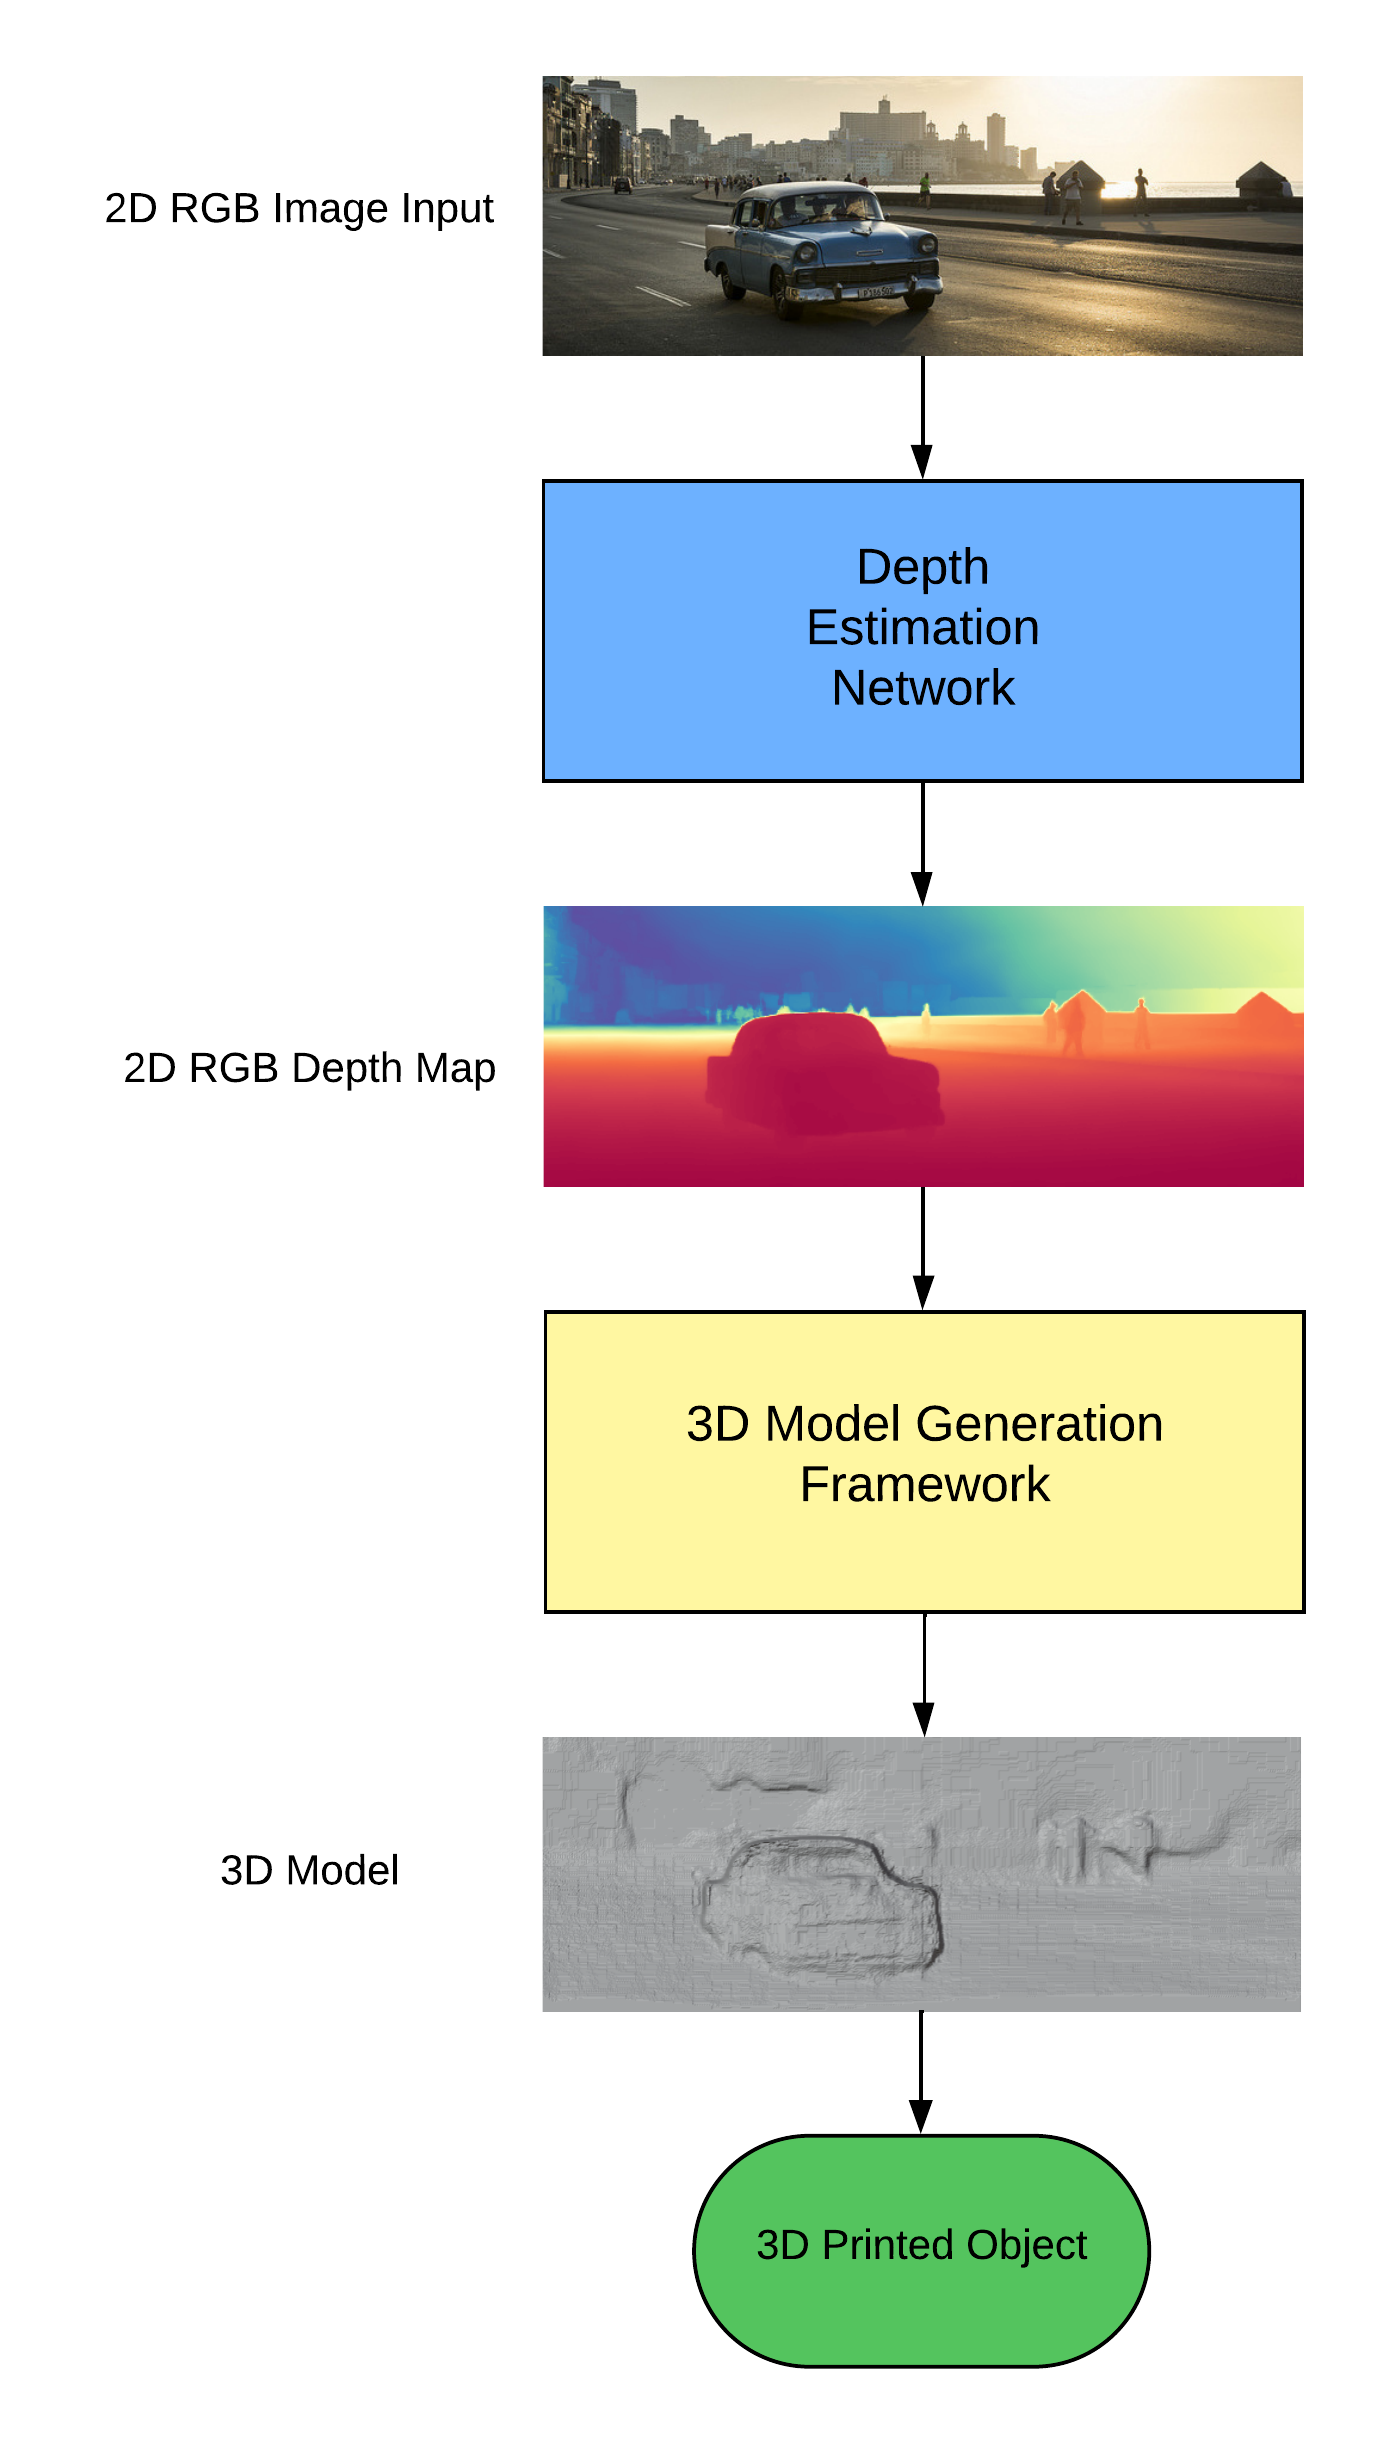
\includegraphics[height = 12.7cm]{framework}
    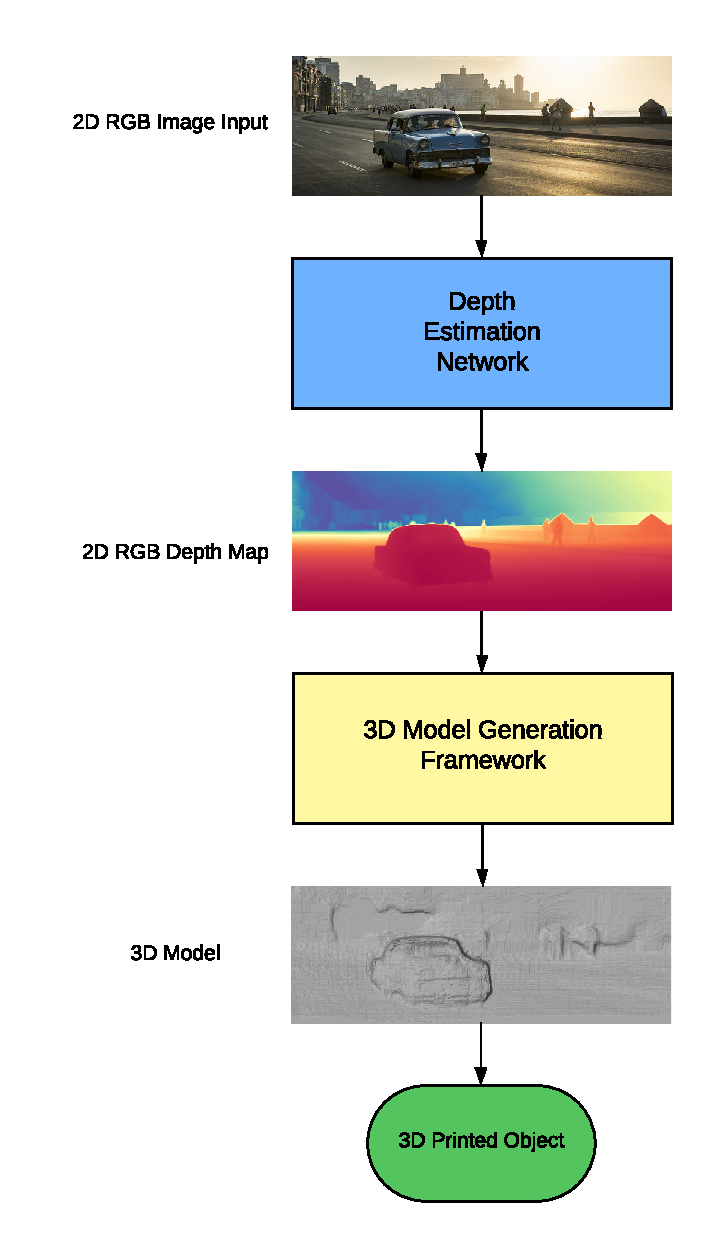
\includegraphics[height = 12.7cm]{pipeline.pdf}
    \caption{Simple pipeline of the proposed method.}
\end{figure}

\subsection{Depth estimation network}
\paragraph{}
To create tactile photos that people with visual impairments can enjoy, the first critical step is generating accurate depth maps from 2D images. This involves using
state-of-the-art depth estimation models that can predict the depth information of each pixel in an image. One of the most advanced models in this area is ``Marigold," \hyperlink{KOH24target}{[KOH24]}
released in 2024, which represents the latest advancements in depth estimation.

\subsubsection{Marigold depth estimation model}
\paragraph{}
The Marigold model leverages diffusion models, specifically Stable Diffusion to achieve high accuracy in depth estimation. It considers the problem of monocular depth estimation as
a conditional denoising diffusion problem. The Marigold model learns to predict depth maps from single RGB images by modeling the conditional distribution \(D(d|x)\) over depth \(d \in \rm I\!R ^{W\times X}\)
given the conditional RGB image \(x \in \rm I\!R^{W\times X \times 3}\) with \textit{W} and \textit{H} the width and height of the image.
The process involves two main phases: the forward and reverse processes.
\begin{enumerate}
    \item Forward process: Gaussian noise is incrementally added to the depth map to obtain noisy samples, starting from the clean depth map conditioned on the RGB image.
    \item Reverse process: The learned denoising model gradually removes noise to obtain a less noisy sample at each iteration. At inference time, the original depth map is 
reconstructed by iteratively applying the learned denoiser.
\end{enumerate}

\paragraph{}
The architecture of the model involves a Variational AutoEncoder (VAE) and a denoising U-Net. The VAE is used to encode the image and its corresponding depth map simultaneously into
a latent space for training the conditional denoiser. The denoising U-Net is conditioned on the input image and its conditioned depth map by concatenating the image and depth latent
codes into a single input.
\paragraph{Fine-tuning}For training, the ground truth depth maps have been normalized in the value range [-1, 1], for two reasons. First because it is the standard for working with Stable Diffusion VAE, and second
because we want to bound the near and far planes with extreme depth values in the image:
\begin{equation}
    \tilde{d} = (\frac{d-d_2}{d_{98}-d_2})\times 2
\end{equation}
where \(d_2\) and \(d_{98}\) are the 2\% and 98\% percentiles of individual depth maps.

Morevover, synthetic datasets are used because they are complete, allowing every pixel having valid ground truth depth values to be fed into the VAE. Indeed, VAE cannot handle data with
invalid pixels, which real depth datasets are full of. The reason for those missing pixels in real depth datasets is due to the physical constraints of the capture device. Reflective
surfaces are a source of ground truth noise and missing pixels.
For the inference, the input image is encoded into the latent space, the depth latent is initialized as standard Gaussian noise and is progressively denoised. Figure \ref{MrgEx} shows achievable results of
accurate depth maps using Marigold.


\begin{figure}[!ht]
    \begin{center}
        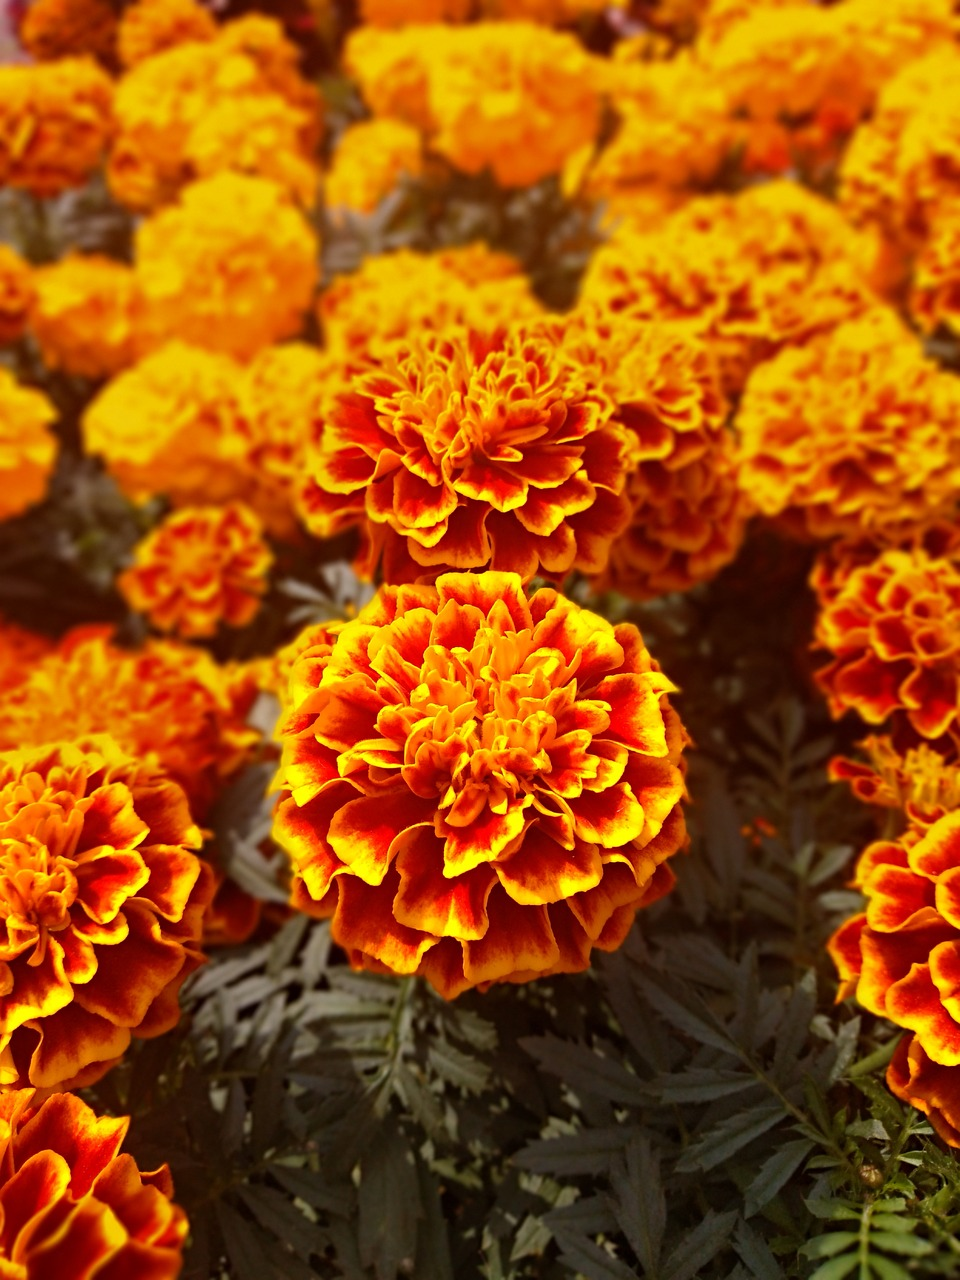
\includegraphics[height = 9cm]{example_0}
        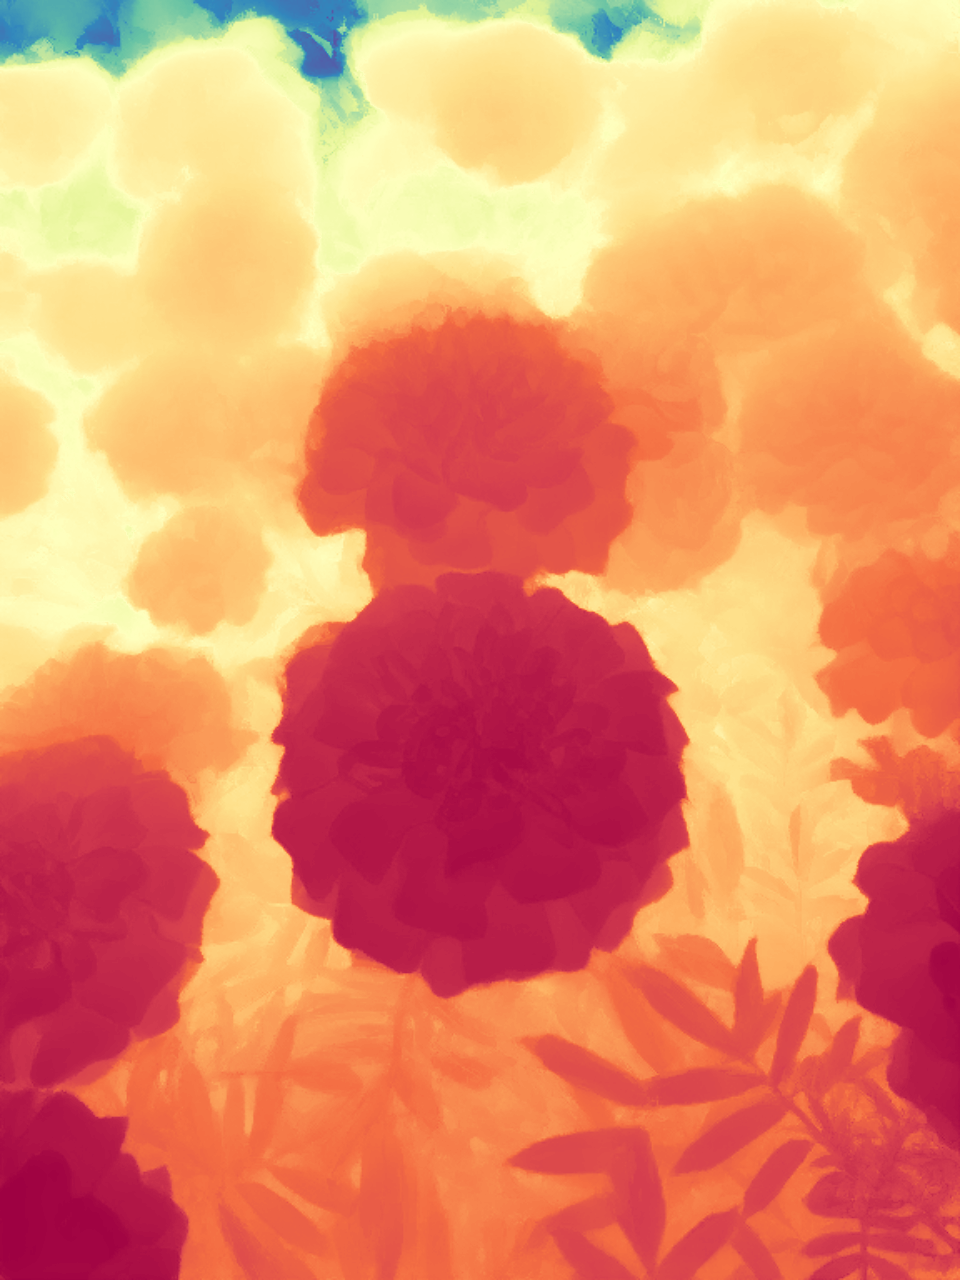
\includegraphics[height = 9cm]{example_0_pred_colored}
        \caption{Example of depth map generated by Marigold.}
        \label{MrgEx}
    \end{center}
\end{figure}

\subsubsection{Self-Reference Distillation}
\paragraph{}

Before adopting the Marigold model, we experimented with the Self Reference Distillation (SRD) method \hyperlink{LRS23target} {[LLS23]}. SRD is a self-supervised learning technique that aims to improve depth estimation by distilling
knowledge from the model itself during training.

The architecture of the SRD model is as follows: the model takes a single RGB image as input and passes through an encoder-decoder network, of which the backbone is a CNN and extracts
features from the input image, ResNet is a network that can be used to extract hierarchical features. After that, the input image is augmented using various transformation, for instance 
scaling or rotation. The augmented images are then passed through the backbone and decoder to generate pseudo-depth labels at different scales.

\begin{figure}[!ht]
    \begin{center}
        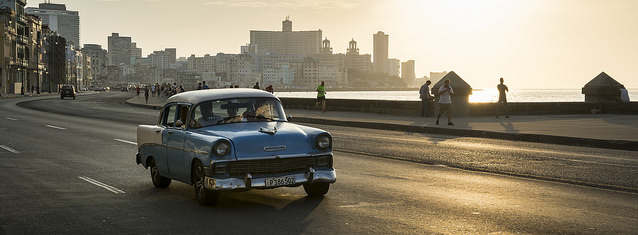
\includegraphics[height = 5cm]{test_image}
        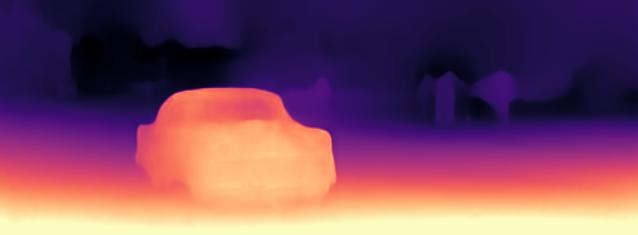
\includegraphics[height = 5cm]{test_image_disp}


        \caption{Satisfing depth map generated using SRD.}
        \label{SRDex}
    \end{center}
\end{figure}

The multiscale output from the encoder is directly input into the decoder, progressively upsampling and convolving the feature maps to increase the resolution. They are then merged with
skip-connected encoding features and passed through layers. A disparity offset is calculated between two adjacent scales, from top to bottom. After the disparity of the original scale is refined,
the decoder outputs disparity and converts it to depth.


\paragraph{}
Even though it seemed satisfying at first, despite its promising approach, the results obtained with SRD were not stable. Figure \ref{SRDex} shows achievable and satisfying results using SRD.
Additionally, compared to the Marigold model, we see that the SRD model struggles in identifying the shapes of each individual object and tends to smooth or spread an object's depth around and
outside its boundaries.
The method involved training a vision transformer to predict depth maps, but the generated depth maps exhibited significant variability, affecting the consistency of the 3D models produced.
Figure \ref{SRDfail} shows some unsuable depth map generated by SRD. This instability led us to explore more robust alternatives, culminating in the adoption of the Marigold model.

\begin{figure}[!ht]
    \begin{center}
        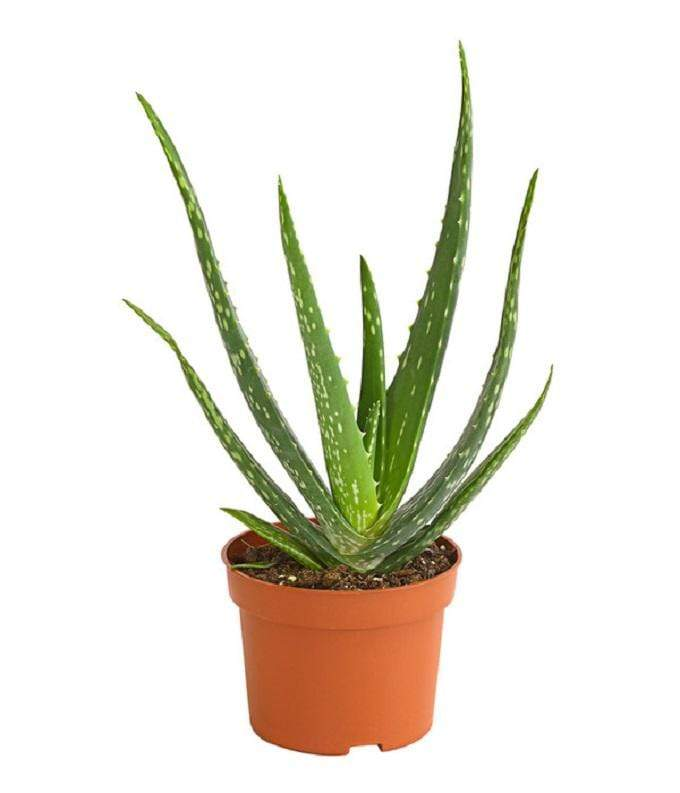
\includegraphics[height = 5.5cm]{jardins-du-senegal-aloe-vera-28830638178417_1200x1200}
        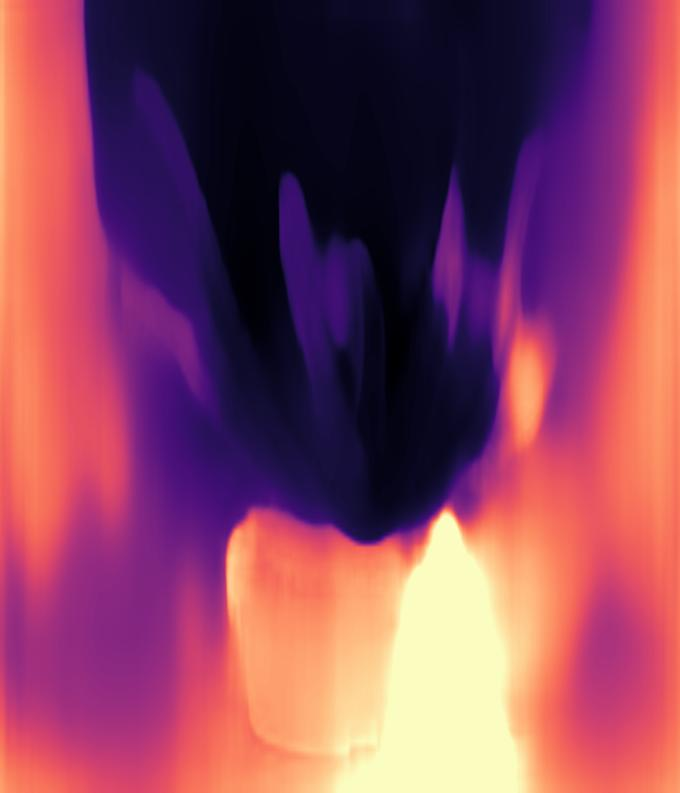
\includegraphics[height = 5.5cm]{jardins-du-senegal-aloe-vera-28830638178417_1200x1200_disp}\\
        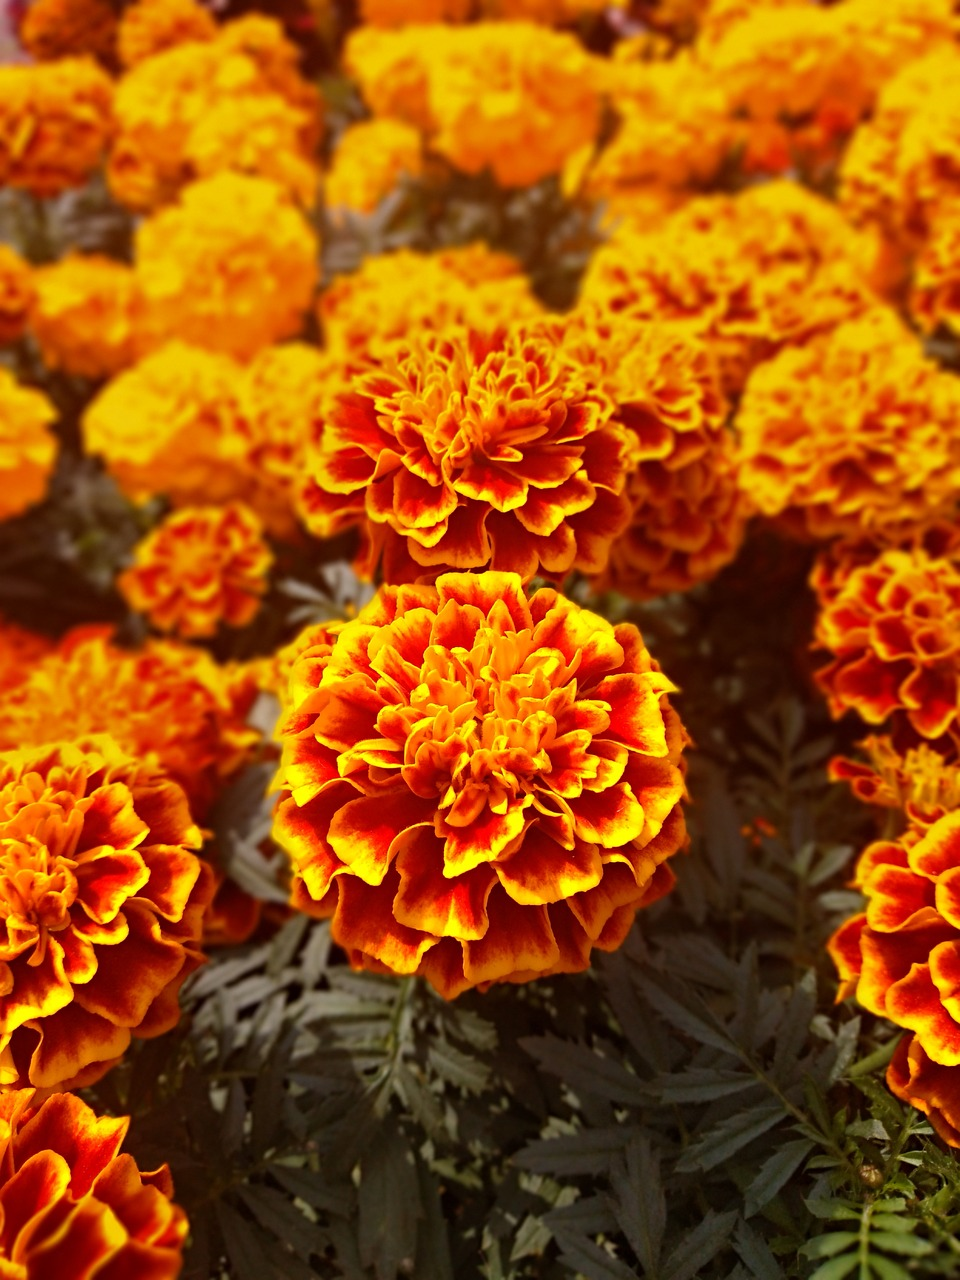
\includegraphics[height = 6.35cm]{example_0}
        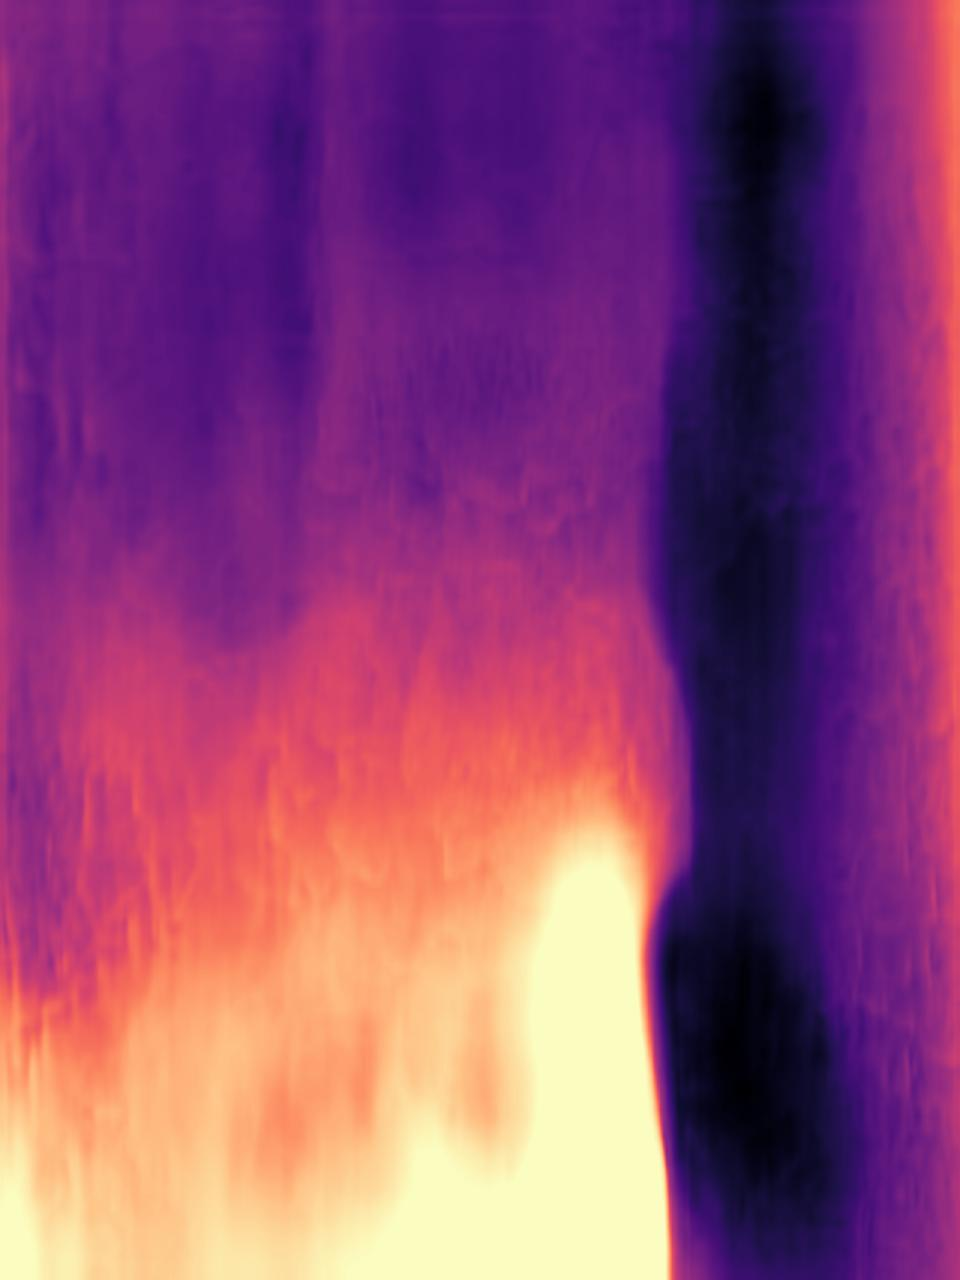
\includegraphics[height = 6.35cm]{example_0_disp}
        \caption{Depth maps generated by SRD for the same input image, which are unusable for the incoming tasks.}
        \label{SRDfail}
    \end{center}
\end{figure}

\subsection{3D reconstruction framework}
\paragraph{}
Once a reliable depth map is obtained using the Marigold model, the next step is to generate a 3D model. This process involves interpreting each pixel in the depth map as
a distance from the viewer, thereby constructing a 3D representation of the scene.
The depth map is essentially either and RGB or a grayscale image where each pixel value represents the distance to the corresponding point in the scene. The colors produced in the case of 
an RGB image depend on the colormap used to generate the depth map. These colormaps include \textit{spectral} or \textit{magma} for example. To convert this into a 3D model:

\paragraph{Depth Map Interpretation} Interpreting a depth map that uses a colormap involves understanding how the colormap maps each depth value to a specific color.
The first approach we used was taking the RGB depth map as it is, and for each pixel, merging the three RGB values into a single one by calculating the mean. This way we would have single depth
values ranging from 0 to 255. Figure \ref{meanapproach} shows results of this approach. Note: this first approach was experimented on using the \emph{SRD} model.

\begin{figure}[ht]
    \begin{center}
        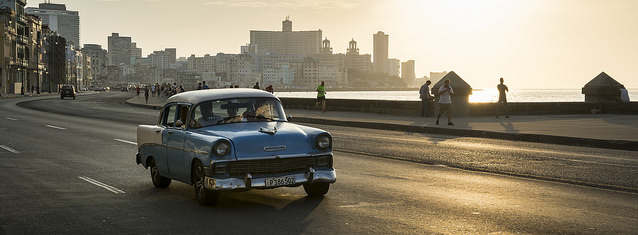
\includegraphics[height = 4.1cm]{test_image}
        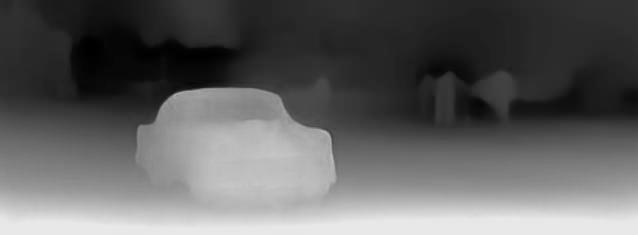
\includegraphics[height = 4.1cm]{test_disp}
        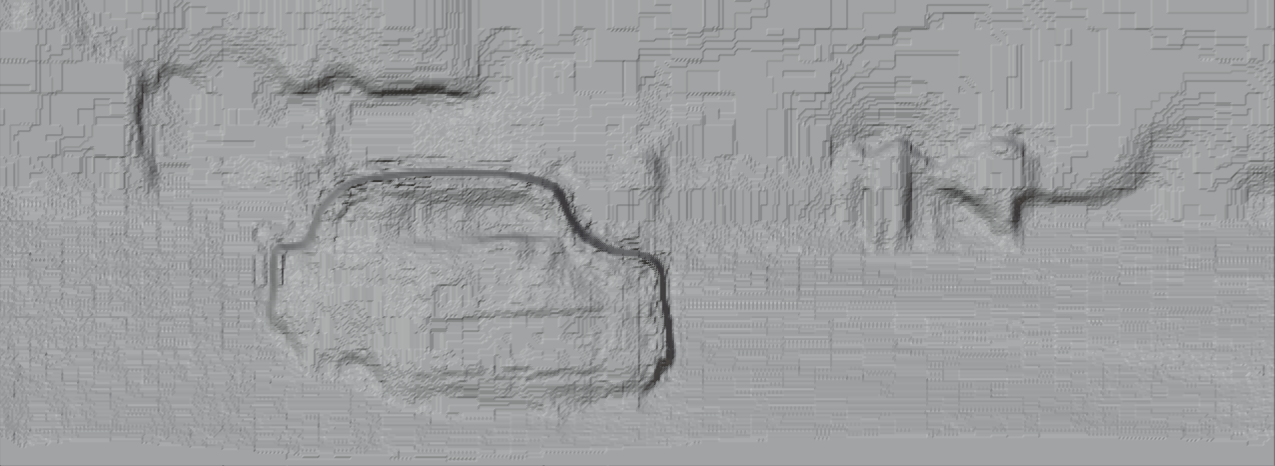
\includegraphics[height = 4.05cm]{3dtest}


        \caption{Interpretation of the values of the depth map by the mean method generted by SRD model.}
        \label{meanapproach}
    \end{center}
\end{figure}

\paragraph{}
In the second and more promising approach, each pixel's RGB value in the depth map is read and is mapped to the values of the colormap. Figure \ref{map} shows the mapping. As shown in Figure \ref{MrgEx},
the pixels are ``the closest" to the camera are red and the ones in the far plane are blue. This way, all the color values that are extracted from the depth map correspond to a value in the
normalized value range [0, 1], with the closest pixels to the camera having the lowest values.

\begin{figure}[ht]
    \begin{center}
        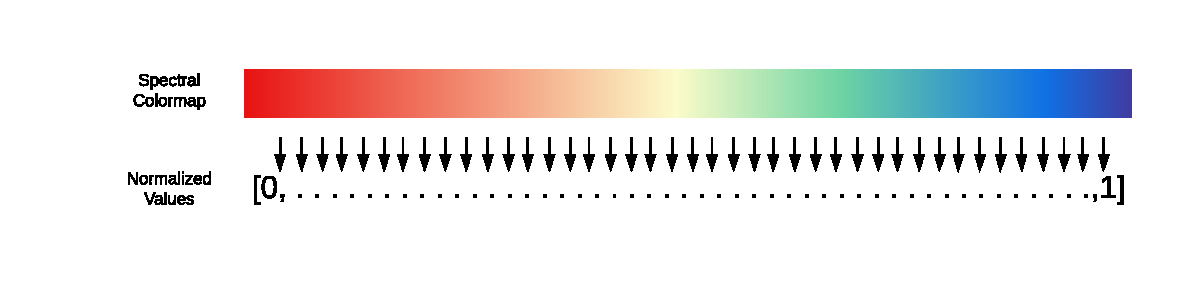
\includegraphics[width=\textwidth]{Mapping.pdf}
        \caption{Mapping of depth values to the colormap, example with Spectral colormap.}
        \label{map}
    \end{center}
\end{figure}

In clear, we convert the RGB values to a range of [0, 1]. We then calculate the Euclidean distance between the given RGB color and all the colors in the colormap that is used, and we find
the index of the closest color. This index is then converted to a normalized depth value by dividing it by the total number of colors in the colormap.

\paragraph{Point Cloud Generation} By combining the x, y, and z coordinates, a point cloud is created, representing the 3D structure of the scene. We go from a \(W\times X\times 3\) array to
a \(W\times X\) array that represents the 3D object. This point cloud serves as the basis for the subsequent steps. Since we want the 3D model to represent the topography of the image, meaning
putting the closest pixel in the image at the highest point in the 3D model when laid down, we need to invert the normalized values. If the values are not inverted, we still get a realistic
topography, but the reproduced 3D model would be a \emph{mirrored} version of the image.

\paragraph{}
We explored emphasizing the closer values and diminishing the far values without erasing them completely. This way, we could focus more on the targeted object in the photo without changing the
composition of the photo in the generated 3D model. In that way, we use some kind of modified \emph{sigmoid} function. We have also explored flattening objects that were below a certain
threshold, but that removes too much information or misrepresents the image, as shown in Figure \ref{Refinements}.
In the end, the emphasis method mentioned previously doesn not change anything much, as shown in Figure \ref{Refinements}. The changes are minor and do not fundamentally change the topology overall.

\begin{algorithm}
    \caption{Point cloud generation algorithm} \label{alg:pointcloud}
    \begin{algorithmic}
        \State $spectralmap \gets RGB depth map$
        \State $colormap \gets colormap\_of\_depth map$
        \State $unique\_colors \gets unique\_color\_of\_spectralmap$
        \For{pixel in spectralmap}
            \State $diff \gets sampled\_colors - pixel$ \Comment{is an array}
            \State $closest\_color\_index \gets minimum(diff)$
            \State $depth[pixel] \gets closest\_color\_index / unique\_colors$

            \State $depth[pixel] \gets depth[pixel]/(1 + e ^ {0.5-5*depth[pixel]})$ \Comment{Experiment, not in final algorithm}
            \State $depth[pixel] \gets 1 - depth[pixel]$
            \If {depth smaller than threshold} \Comment{Experiment, not in final algorithm}
                \State $depth[pixel] \gets 0$
            \EndIf
        \EndFor
        \State{return $depth$}
    \end{algorithmic}
\end{algorithm}


\paragraph{Mesh Construction} The point cloud is then converted into a mesh, a collection of vertices, edges, and faces that define the shape of the 3D model. As mentioned previously, we
want the 3D model to be usuable in the educational field. At the same time, we want it not to be too thick so that it is storable. In that way, we decided to give it an \emph{A4} format, that
is to say $21cm\times29.7cm\times5cm$ dimensions.
\paragraph{}
To do so, we use specific libraries available in \emph{Python}, such as \emph{PILLOW} and \emph{numpy-stl}. In the latter library, we can use the \emph{mesh} function to construct the 3D object.
It takes an array of faces to create the vectors that compose the 3D object. To construct those faces which are actually trigons, if we consider $i$ and $j$ respectively a row and column index,
we iteratively take the $(i,j)-th$, $(i+1,j)-th$, and \emph{(i, j+1)-th} vertices on one hand, $(i+1,j)-th$, $(i,j+1)-th$, and $(i+1, j+1)-th$ on another and link them to create 2 distinct
but trigons. Additionally, the vertices are not represented as a 2-dimensional array that stores the depth values, but rather a \((W*H) \times 3\) array, with each cell of the array being stored
as \([x, y, d]\). We detail the algorithm in Algorithm \ref{alg:3d}

\begin{algorithm}
    \caption{3D mesh generation} \label{alg:3d}
    \begin{algorithmic}
        \State $image \gets RGB depth map$
        \State $x,y \gets dimensions(image)$

        \For{i in x}
        \For{j in y}
            \State $vertices[(i*y+j)] \gets [i, j, img[i, j]]$
        \EndFor
        \EndFor

        \For{i in x-1}
        \For{j in y-1}
            \State $faces.append([j + i*y, j+1 + i*y, j+(i+1)*y])$
            \State $faces.append([j+1 + i*y, j + (i+1)*y, j+1 +(i+1)*y])$
        \EndFor
        \EndFor
        
        \For{i, f in enumerate(faces)}
            \For{j in range 1 to 3}
                \State $mesh3d.vectors[i][j] \gets vertices[f[j], :]$ \Comment{Specific \emph{numpy-stl} function}
            \EndFor
        \EndFor

    \end{algorithmic}
\end{algorithm}

\paragraph{} Moreover, as mentioned previously, we want the resulting 3D model to have specific dimensions, that is to say $21cm\times29,7cm\times5cm$. Initially, after passing through Algorithm
\ref{alg:3d}, the scale of the 3D model is in meters, so we need to multiply the values of the 3D model by a \emph{scaling factor}.
In terms of length by width ratio, the desired dimensions $21cm\times29,7cm\times5cm$ represents around \emph{1.414}. However, the input image does not necessarily respect this ratio, but
we want it to \underline{fit} within these dimensions. To do that, we need to identify wether the image is in portrait or landscape orientation (if it is in portrait orientation, then
there are more rows than columns in the input image, and vice versa). Then we check if its ratio is greater or smaller than $1.414$. If that is the case, then it means that we need to set the model size
so that its longest portion's length is equal to \(29.7cm\). If not, we do it so that its shortest portion's length is equal to $21.0cm$. In sum, we ensure that at least one of the 3D printed
object's side matches either the $21.0cm$ or $29.7cm$ length. Figure \ref{resize} illustrates how the scaled image would fit within the desired dimensions.

\begin{figure}[!ht]
    \begin{center}
        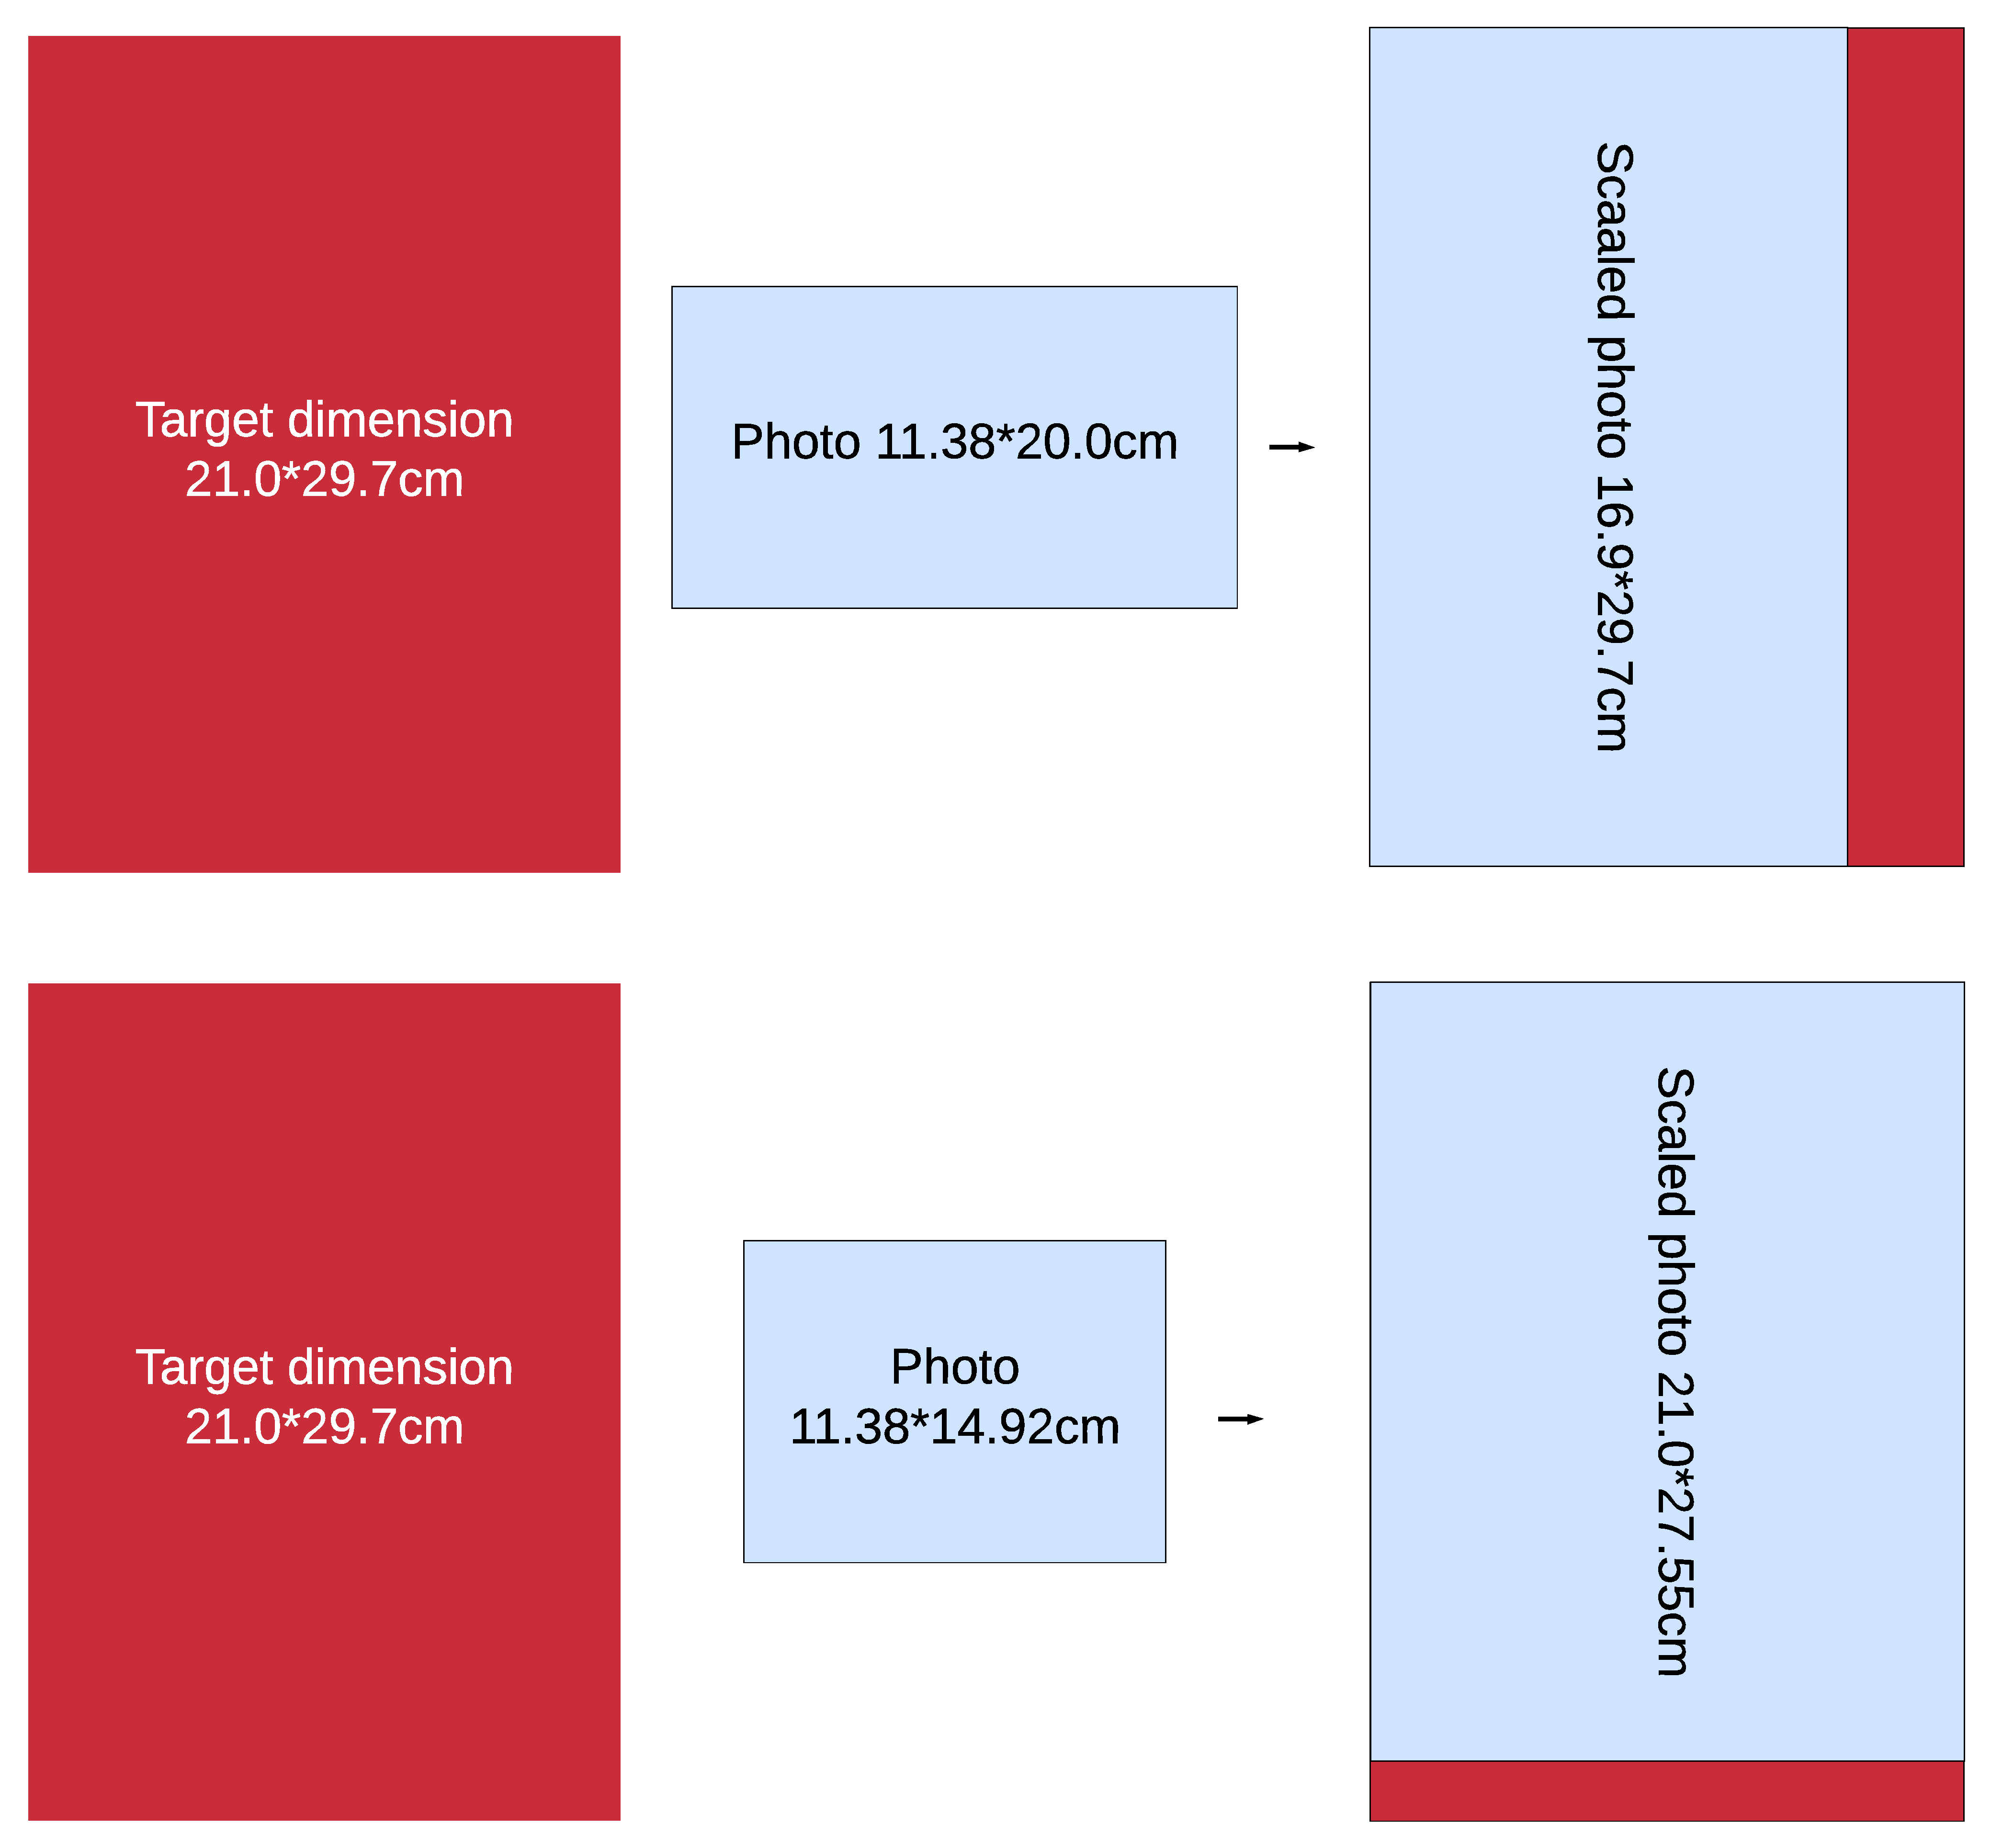
\includegraphics[height = 11cm]{resize.pdf}
        \caption{Scaling the 3D model so that it fits within an A4 paper ($21cm\times29,7cm\times5cm$).}
        \label{resize}
    \end{center}
    \small
    In this example, we show how two photos of different ratios (one above $1.414$ and one below) would fit within the desired dimensions. As we see in
    the two examples, the rescaled 3D model would leave a bit of unused space, maintaining the original ratio of the image.
\end{figure}

\paragraph{}
In clear, we first check if the input image is in portrait or landscape mode, afterwards we check the length over width ratio of the image to check if it is smaller or 
bigger than the desired ratio $1.414$. If we consider $x, y$ the horizontal and vertical length values of the image, we calculate the scaling factor (a three-dimensional value $[x, y, z]$) 
according to these conditions:
\begin{enumerate}
    \item Portrait: if the ratio is smaller than $1.414$, the scaling factor is

    \([0.297/y, 0.297/y, 0.05]\). Otherwise, it is equal to $[0.21/x, 0.21/x, 0.05]$

    \item Landscape: if the ratio is smaller than $1.414$, the scaling factor is

    \([0.21/y, 0.21/y, 0.05]\). Otherwise, it is equal to $[0.297/x, 0.297/x, 0.05]$
\end{enumerate}

After getting the scaling factor for each $x, y$, and $z$ axis, we multiply the mesh by the scaling factor axis-wise to get the A4 scaled mesh.

\paragraph{3D Printing Preparation} The final mesh is then prepared for 3D printing. This involves optimizing the model to ensure it can be printed accurately, considering factors like
the resolution and capabilities of the 3D printer. By following these steps, we can generate highly detailed and accurate 3D models from depth maps, which can be transformed into
tactile photos. These tactile photos enable individuals with visual impairments to perceive and enjoy visual content through touch, significantly enhancing their accessibility to visual
information.

\subsection{Conclusion}

\paragraph{}
In this chapter, we have presented a comprehensive method for enabling visually impaired individuals to create tactile 3D representations of photos they have taken or provided as input.
By leveraging state-of-the-art depth estimation models, such as the Marigold model, our approach effectively translates 2D images into depth maps that accurately capture the topography of
the scene. These depth maps are then interpreted and converted into 3D models suitable for printing using a 3D printer.
\paragraph{}
The process begins with the Marigold model, which uses advanced diffusion techniques to generate depth maps from single RGB images, ensuring high accuracy and consistency. This model was
chosen after evaluating alternatives like the Self-Reference Distillation (SRD) method, which, while promising, did not provide the reliability needed for our application. The depth maps
generated are then interpreted to create point clouds, which form the basis of the 3D models. Special attention is given to accurately mapping depth values and ensuring that the tactile
models convey the intended topographical features.
\paragraph{}
Through this method, we have developed a pipeline that not only allows for the creation of 3D tactile photos but also ensures that these models are meaningful and accessible to visually
impaired users. The final 3D models are supposed to maintain the integrity of the original images' composition while emphasizing the depth features necessary for tactile exploration.
This work lays the groundwork for future advancements in making visual content more accessible through touch, providing a valuable tool for enhancing the sensory experiences of visually impaired individuals.

\newpage

%%%%%%%%%%%%%%%%%%%% RESULTS %%%%%%%%%%%%%%%%%%%%%%%%
\section{Results}
\subsection{Self-Reference Distillation}

\paragraph{}
As mentioned in Chapter 3, we have used the Self Reference Distillation model in the first place. This sub section will display the capabilities of the model through generated depth maps
and associated generated 3D models.

\paragraph{}
The first image we have tested the protocol on was available in the model's project github called \emph{test\_image} that supposedly showcases what the model does to its
full extent.

\begin{figure}[!ht]
    \begin{center}
        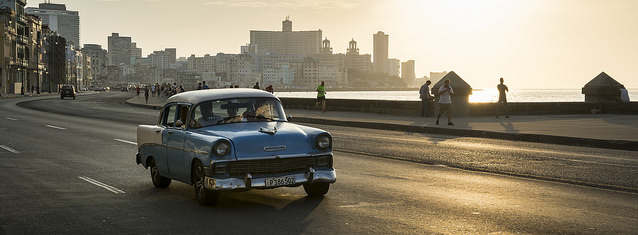
\includegraphics[height = 3cm]{test_image}
        \caption{test\_image as provided.}
        \label{testimg}
    \end{center}
\end{figure}

\paragraph{}
As a first approach, prior to thinking of interpreting the depth map, we thought of calculating the mean value of each pixel, so that instead of having three dimensional
values, we would have one dimensional values that would directly be used as depth values. But with this approach we only get 256 different depth values, which does not seem
optimized for realistic reconstruction. Figure \ref{SRDcompare} shows the difference in the two approaches along with their reconstructed 3D models for the test\_image.
\paragraph{}
The differences are minor but we can see that with the model generated from the mean approach (black and white), the topography is less smooth and more chunky as compared to the one
that was generated using the RGB depth map. As explained previously, this is due to the fact that there are more possible depth values in the RGB depth map than in the black and white depth map, which is natural.

\begin{figure}[!ht]
    \begin{center}
        \begin{subfigure}[b]{0.45\textwidth}
            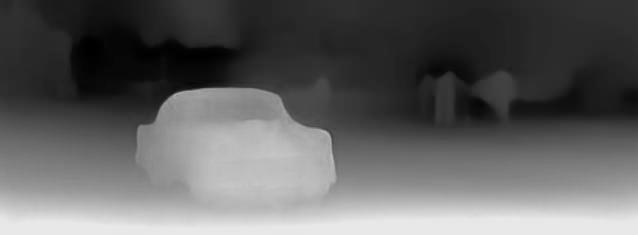
\includegraphics[height = 2.5cm]{test_disp}
            \caption{}
        \end{subfigure}
        \begin{subfigure}[b]{0.45\textwidth}
            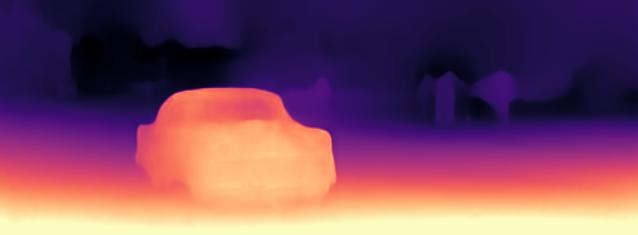
\includegraphics[height = 2.5cm]{test_image_disp}
            \caption{}
        \end{subfigure}
        \begin{subfigure}[b]{0.45\textwidth}
            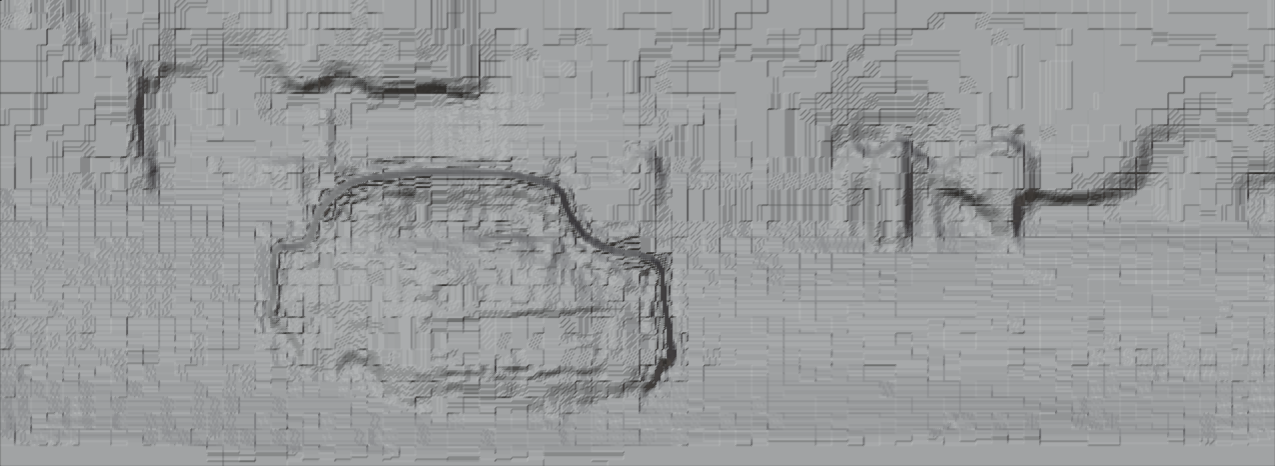
\includegraphics[height = 2.49cm]{3d_bw_depth}
            \caption{}
        \end{subfigure}
        \begin{subfigure}[b]{0.45\textwidth}
            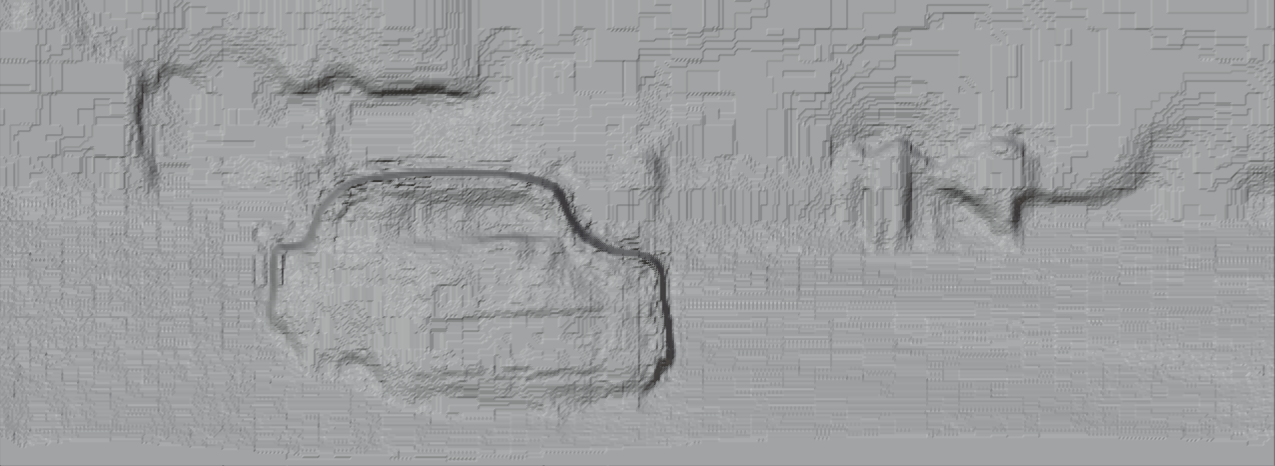
\includegraphics[height = 2.49cm]{3dtest}
            \caption{}
        \end{subfigure}
        \caption{Results of mean depth values compared to RGB values.}
        \label{SRDcompare}
    \end{center}
    \small
    This figure presents the results of a mean-interpreted depth map (a) as compared to a RGB depth map (b), using the \emph{magma} colormap in this case - as well as their
    generated 3D model (c) and (d), using the protocol described in the \emph{Proposed method}. The 2 depth maps here are generated using the SRD model.
\end{figure}

\vspace{3cm}
\paragraph{}
To enhance the usability and tactile clarity of the models, and highlight the difference between close and far objects, we tried further refinements, such as adjusting the depth values
using a modified sigmoid function or deleting objects that were below a certain depth value threshold. Figure \ref{Refinements} shows the results of these refinements attempts.

\begin{figure}[!ht]
    \begin{center}
        \begin{subfigure}[b]{0.45\textwidth}
            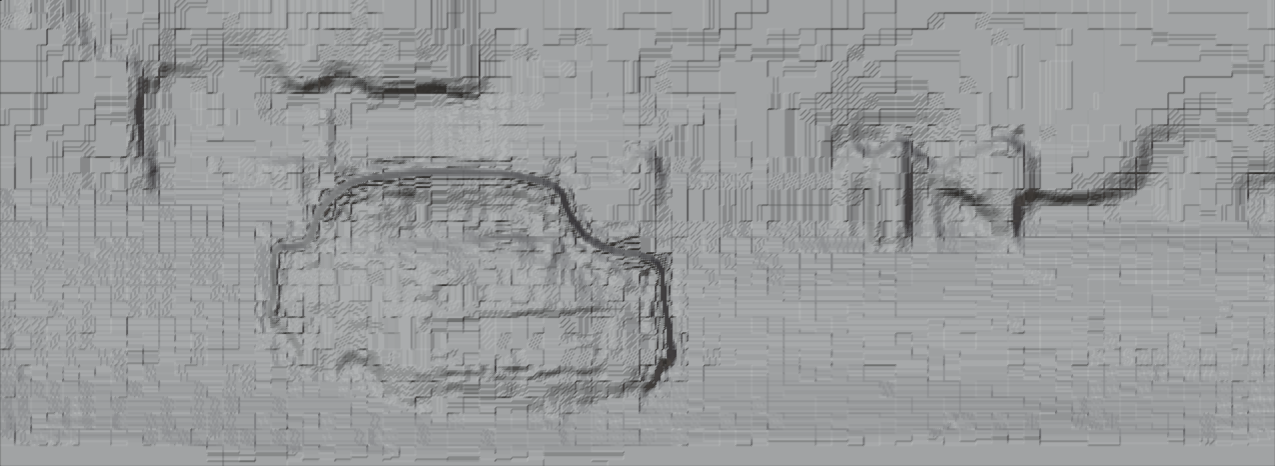
\includegraphics[height = 2.49cm]{3d_bw_depth}
            \caption{}
        \end{subfigure}
        \begin{subfigure}[b]{0.45\textwidth}
            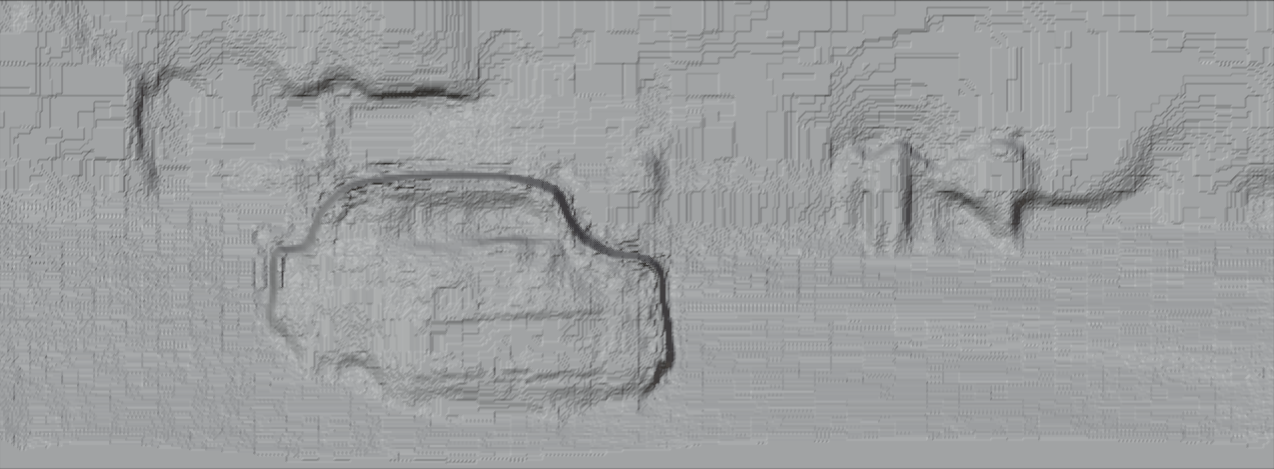
\includegraphics[height = 2.5cm]{3d_bw_depth_emph}
            \caption{}
        \end{subfigure}
        \begin{subfigure}[b]{0.45\textwidth}
            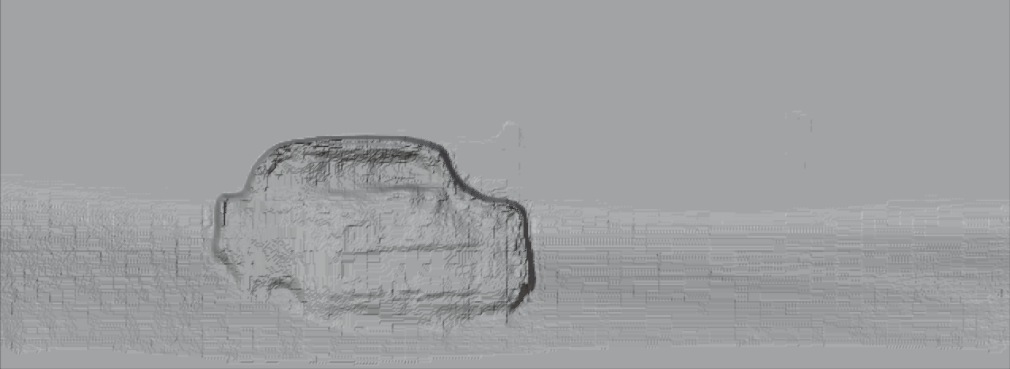
\includegraphics[height = 2.49cm]{low_rm}
            \caption{}
        \end{subfigure}
        \begin{subfigure}[b]{0.45\textwidth}
            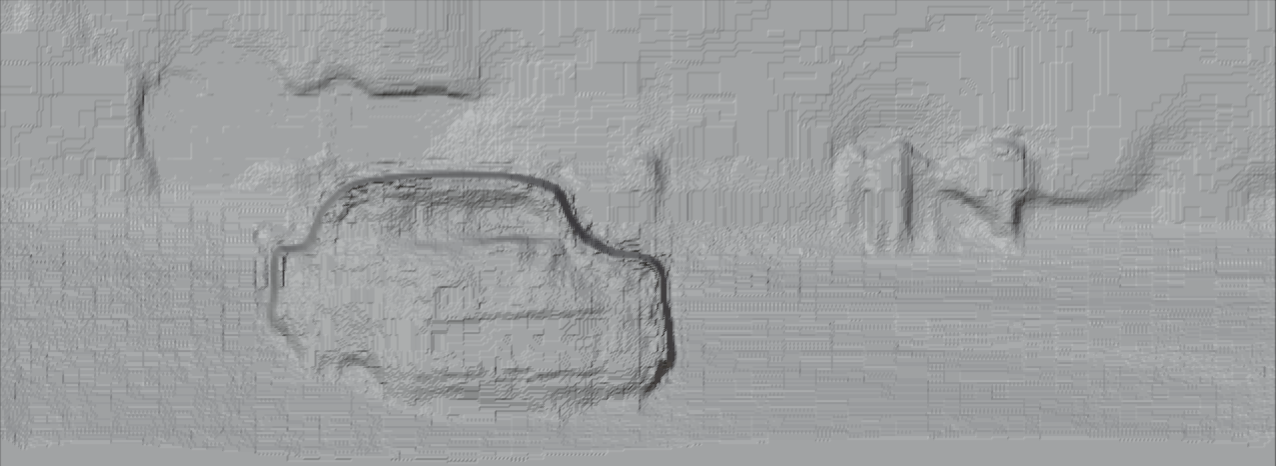
\includegraphics[height = 2.49cm]{low_rm2}
            \caption{}
        \end{subfigure}


        \caption{Results of refinements.}
        \label{Refinements}
    \end{center}
    \small
    This figure presents the results of a the refinements. The first image \emph{(a)} is the 3D model generated without any refinement. The second image \emph{(b)} has the sigmoid function
    applied to it. In the third image \emph{(c)}, the threshold is set to $0.2$ and $0.05$ in the last image \emph{(d)}.
\end{figure}

\paragraph{Failures} We have decided to move onto another model after encountering problems with the generation of depth map. We noticed that the model first struggled in delimiting individual
objects. It tends to spread and blend one's object depth to others if they are deemed close by the model. Though the depths seem accurate, especially for objects close to the camera, the model
struggles in capturing the actual shape of the objects as objects that are past a certain distance threshold are barely recognizable (see Figures \ref{SRDcompare} and \ref{appSRD}).
Ultimately, the model does not find any solution if the input image has too many objects or is too detailed (see Figure \ref{appSRD}).

\subsection{Marigold}

\begin{figure}[hb]
    \begin{center}
        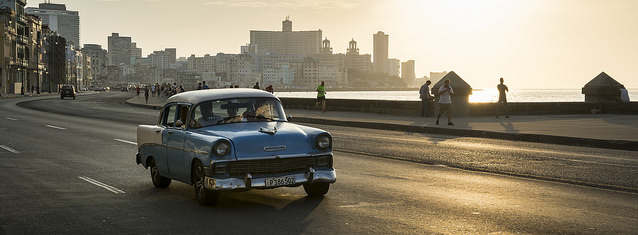
\includegraphics[scale = .33]{test_image}
        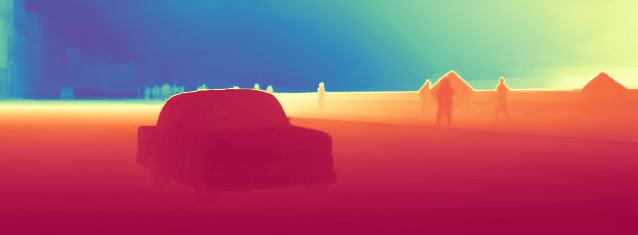
\includegraphics[scale = .33]{test_image_pred_colored}
        \caption{Result of depth map generated by Marigold.}
        \label{MRGres}
    \end{center}
\end{figure}

\paragraph{}
Here, we present the results obtained from applying the Marigold depth estimation model to generate depth maps from 2D images, which were then used to create 3D printable models.
The aim was to evaluate the accuracy and effectiveness of the Marigold model in producing depth maps that faithfully represent the topographical features of input images, and to assess
the tactile usability of the resulting 3D models. Considering the results obtained with the Self Reference Distillation model, we have decided to move onto this instead, which is more recent and provides more
convincing and tangible results.

\paragraph{}
We apply the Marigold model to a set of diverse input images, ranging from simple objects to complex scenes. The model successfully generated depth maps that captured detailed depth
variations across different objects and surfaces in each image. Figures \ref{MRGres} and \ref{compSRDMRG} show examples of depth maps generated from different input images. In these figures, depth is represented
by a gradient of values called \emph{Spectral}, where red shades correspond to areas closer to the viewer and blue shades represent areas farther away, while yellow shades correspond to areas
in between.

\paragraph{}
The depth maps produced by the Marigold model demonstrated a high level of detail and accuracy in distinguishing between different objects and their relative distances.
This was particularly evident in images with varying depths, where the model accurately represented the spatial relationships between foreground and background elements.
The model was also able to handle complex textures and subtle depth variations, resulting in depth maps that closely mirrored the actual depth information of the scenes.

\paragraph{}
Following the generation of depth maps, these were interpreted to create 3D models. As expalined in the \emph{Depth map interpretation} section of the proposed method, the
depth values were mapped to a normalized range, and each pixel was converted into a corresponding point in a 3D space. The resulting point clouds were then processed to form
continuous surfaces, effectively translating the depth information into tangible 3D topographies.

\begin{figure}[t]
    \begin{center}
        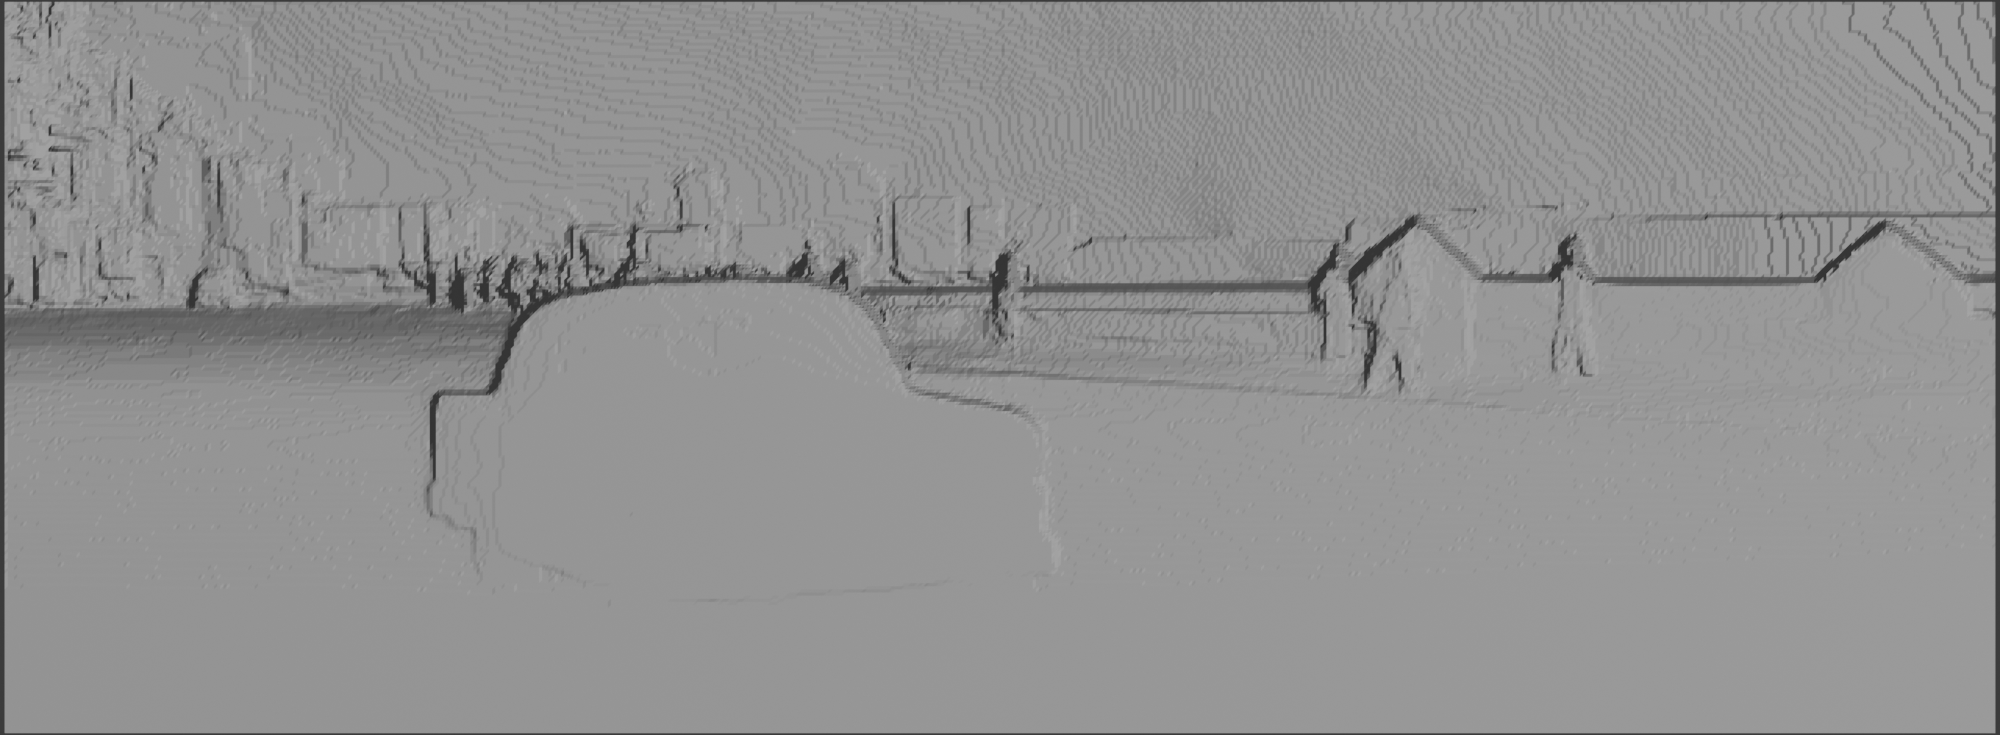
\includegraphics[height = 5cm]{test_image_pred_colored3d}
        \caption{3D model produced using a depth map generated by Marigold.}
        \label{MRG3D}
    \end{center}
\end{figure}

Figure \ref{MRG3D} present the 3D model generated from the depth map of the image shown in Figure \ref{MRGres}. These models were evaluated based on their structural
integrity and the fidelity with which they represented the original images' topographical features as they effectively highlighted the depth variations, with closer objects
being elevated and distant objects being recessed, thus creating a tactile representation of the scene.

\subsection{Comparing SRD and Marigold}

\begin{figure}[!ht]
    \begin{center}
        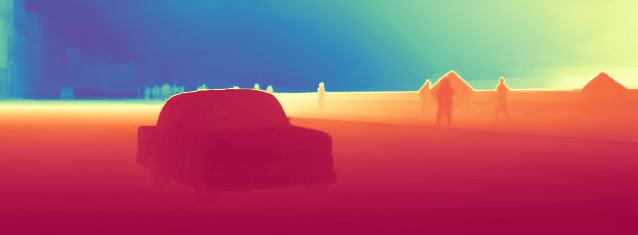
\includegraphics[height = 2.5cm]{test_image_pred_colored}
        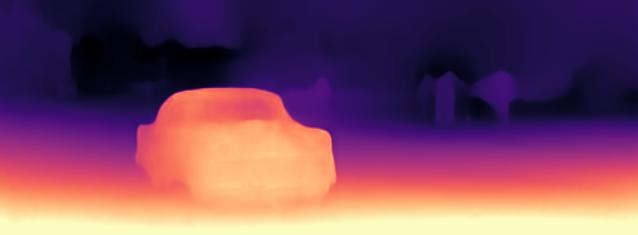
\includegraphics[height = 2.5cm]{test_image_disp}\\
        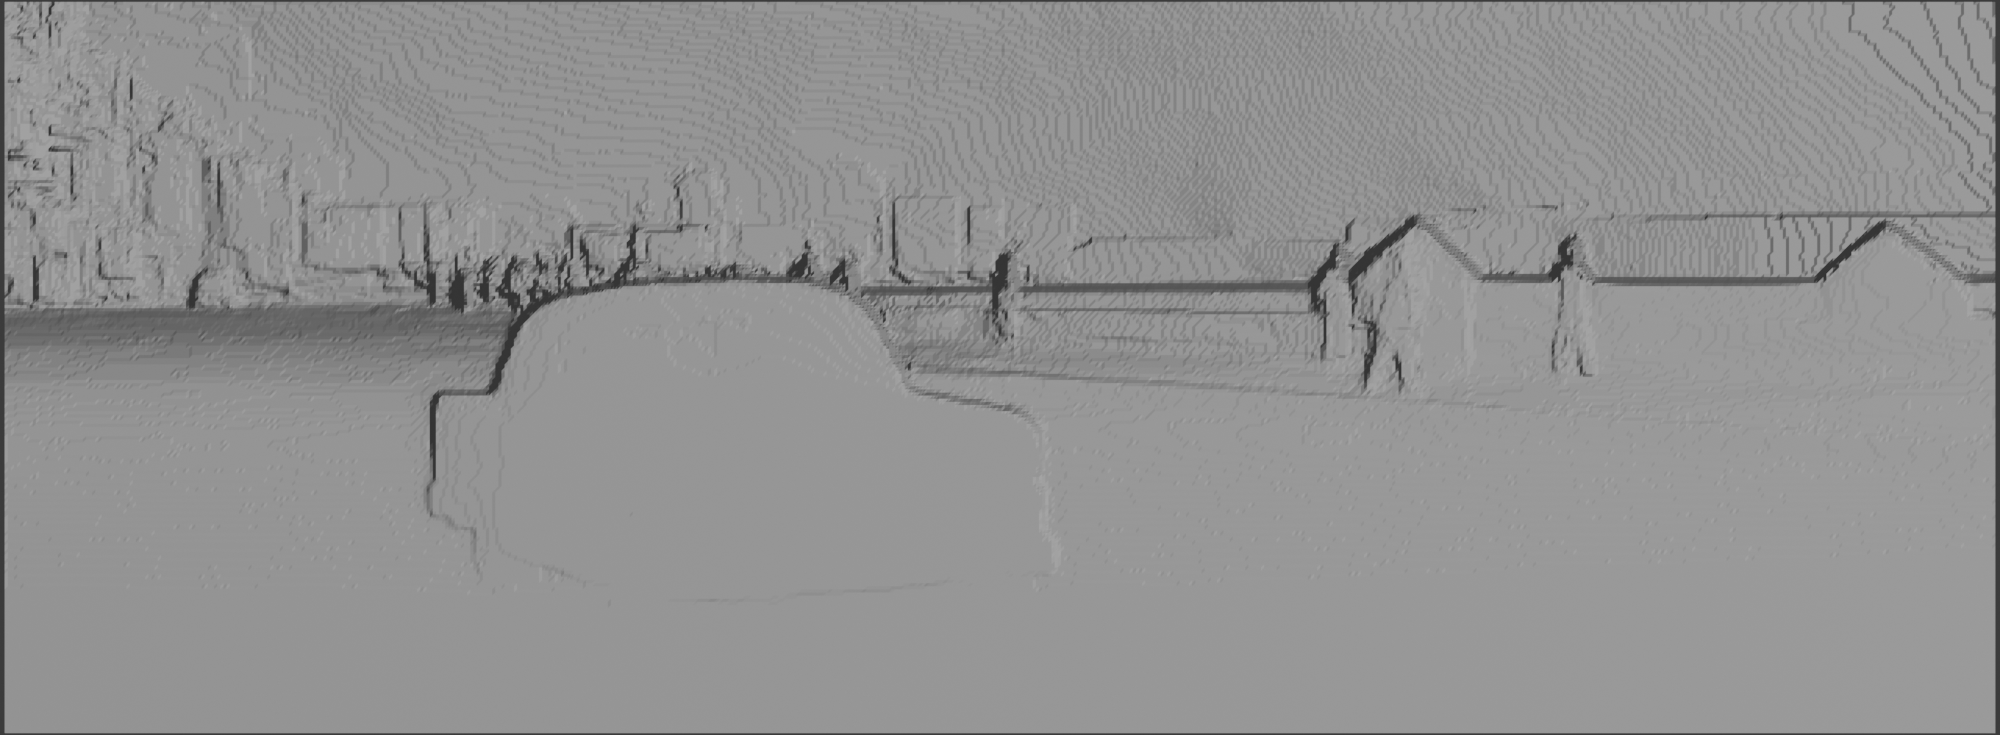
\includegraphics[height = 2.49cm]{test_image_pred_colored3d}
        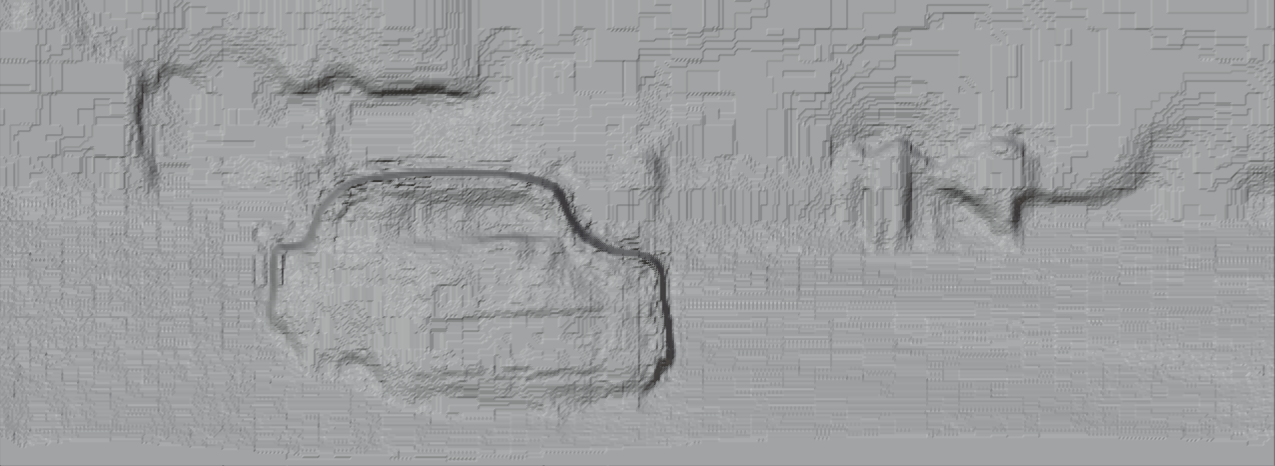
\includegraphics[height = 2.49cm]{3dtest}


        \caption{Comparing the resulting 3D model for the same input image.}
        \label{comparison}
    \end{center}
    \small
    First column is the Marigold generated depth map and its corresponding 3D model, second column is obtained with SRD.
\end{figure}

\paragraph{}
To provide a comparative analysis, the results obtained using the Marigold model were contrasted with those from the SRD model, which was
initially considered for this task. While the SRD model was capable of generating depth maps, the results were
inconsistent, with significant variability in the depth values across similar scenes. This inconsistency led to 3D models that lacked
the structural coherence necessary for effective tactile exploration, as demonstrated in Figure \ref{comparison}.

\paragraph{}
In contrast, the Marigold model consistently produced depth maps that translated into reliable and detailed 3D models.
The comparison highlighted the superior stability and accuracy of the Marigold model, making it the preferred choice for this application.
The Marigold-generated models were free from the smoothing artifacts observed in the SRD results, which often blurred the boundaries between
distinct objects, leading to supposedly less informative tactile models.

\subsection{Complexity of the process}

\paragraph{} The produced 3D models may seem satisfying from a reconstruction point of view, but computationally they are way too demanding. Table \ref{table:timeelapsed} gives
information on the time taken to generate 3D models depending on the image's resolution, as well as the number of vertices and faces it contains.\\

\begin{table}[th!]
\begin{center}
    \begin{tabular}{ | m{3.5cm} | >{\raggedleft\arraybackslash}m{3.5cm}| >{\raggedleft\arraybackslash}m{3.5cm} | >{\raggedleft\arraybackslash}m{2.8cm} | } 
    \hline
    Image size in pixels & Number of vertices & Number of faces & Time elapsed \\ 
    \hline
    \hline
    $235 \times 638$ & 149,930 & 298,116 & 4.7 seconds\\ 
    \hline
    $539 \times 719$ & 387,541 & 772,568 & 11.8 seconds\\ 
    \hline
    $1280 \times 960$ & 1,228,800 & 2,453,122 & 38.8 seconds\\  
    \hline
    $3648 \times 2736$ & 9,980,928 & 19,949,090 & 336.1 seconds\\  
    \hline
    $4160 \times 5547$ & 23,075,520 &  & 714.1 seconds\\  
    \hline
    \end{tabular}
    \small
    Note : The computer provided by the laboratory was not powerful enough to display the last 3D model in the render software, which is the reason we do not have
    information on the number of faces.
    \caption{Data on the generated 3D models}
    \label{table:timeelapsed}
\end{center}
\end{table}

To address this complexity issue, we have tried reducing the number of vertices, reducing the number of faces accordingly. However we could not find a means to perform the process
at the same time as the protocol previously mentioned, so the \emph{decimation} is done post-processing and adds computation time, though it gives a rough idea of what degree of
simplification is achievable in that way.

\begin{figure}[!ht]
    \begin{center}
        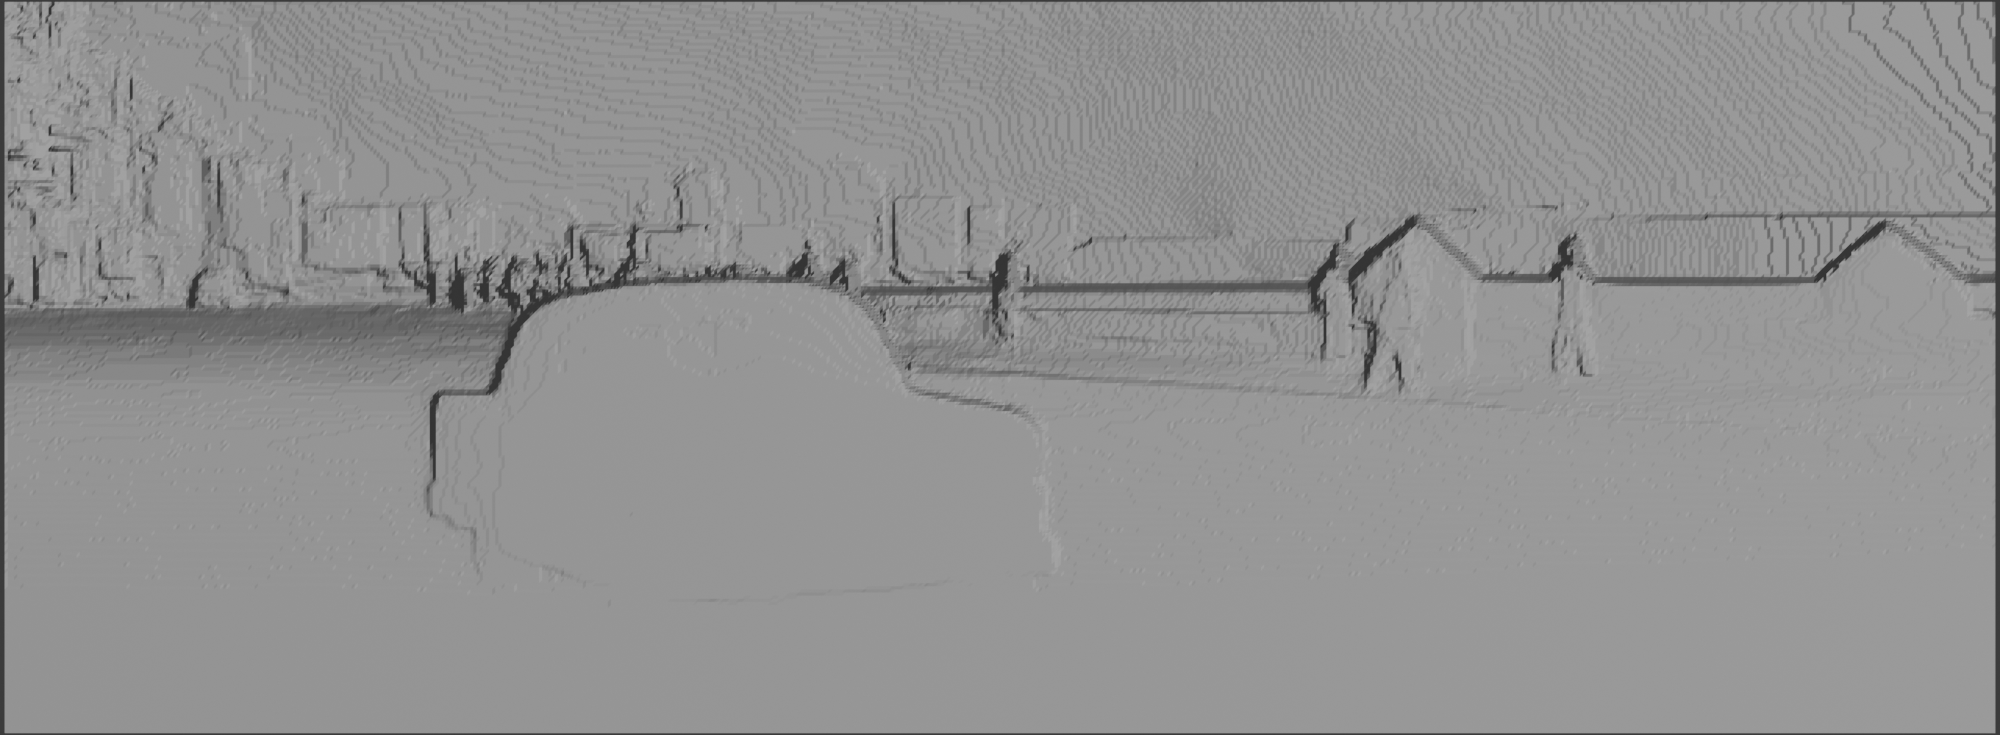
\includegraphics[height = 4cm]{test_image_pred_colored3d}
        
\includegraphics[height = 4cm]{test_image_pred_colored_3d_50}
        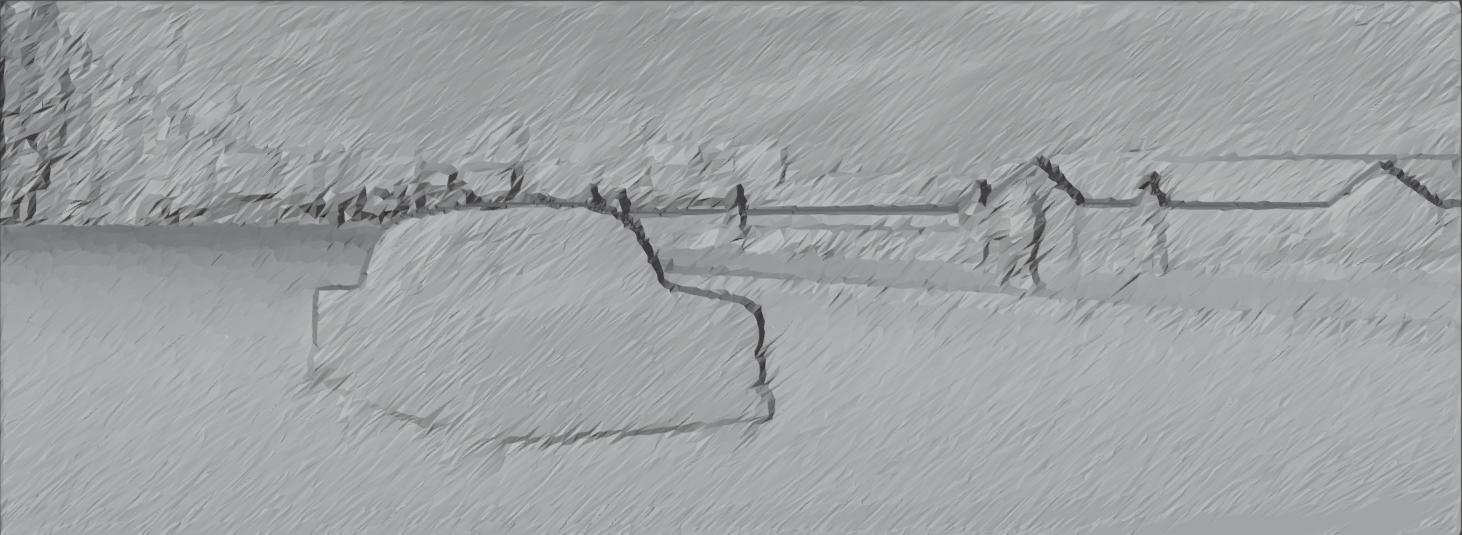
\includegraphics[height = 4cm]{test_image_pred_colored_3d_90}


        \caption{Result of decimation.}
        \label{decimation}
    \end{center}
    \small
    The first image is the original 3D model without decimation applied, the second one has a 50\% decimation rate, and the last one a 90\%
    decimation rate. This means that the first model contains 149,930 vertices, against 74,965 and 14,993 for the second and third respectively.
    We also go from X faces for the first to Y for the second, and Z for the third.
\end{figure}

It also remains to be seen if these decimated 3D models can still be understood by people with visual impairments, and to what extent. As we can see on Figure 
\ref{decimation}, the decimated models seem rough, which can be uncomfortable to the touch, something to be valued.


\clearpage
\newpage


%%%%%%%%%%%%%%%%%%%% DISCUSSION %%%%%%%%%%%%%%%%%%%%%%%%
\section{Discussion and continuation}

\subsection{Further work}

\paragraph{Sky segmentation} It would be interesting to identify scenes where the sky is part of the photo, and if the focus is effectively on the sky and its components or not, for instance a 
photo of a plane flying or hot-air balloon festival. If the sky is not an essential part of the photo, in the final printed object, it would not be removed - though its information
is not relevant compared to other objects present in the scene, it is still interesting to keep it. The sky's depth would be set to 0 and it would be a flat surface in the back.

\begin{figure}[!ht]
    \begin{center}
        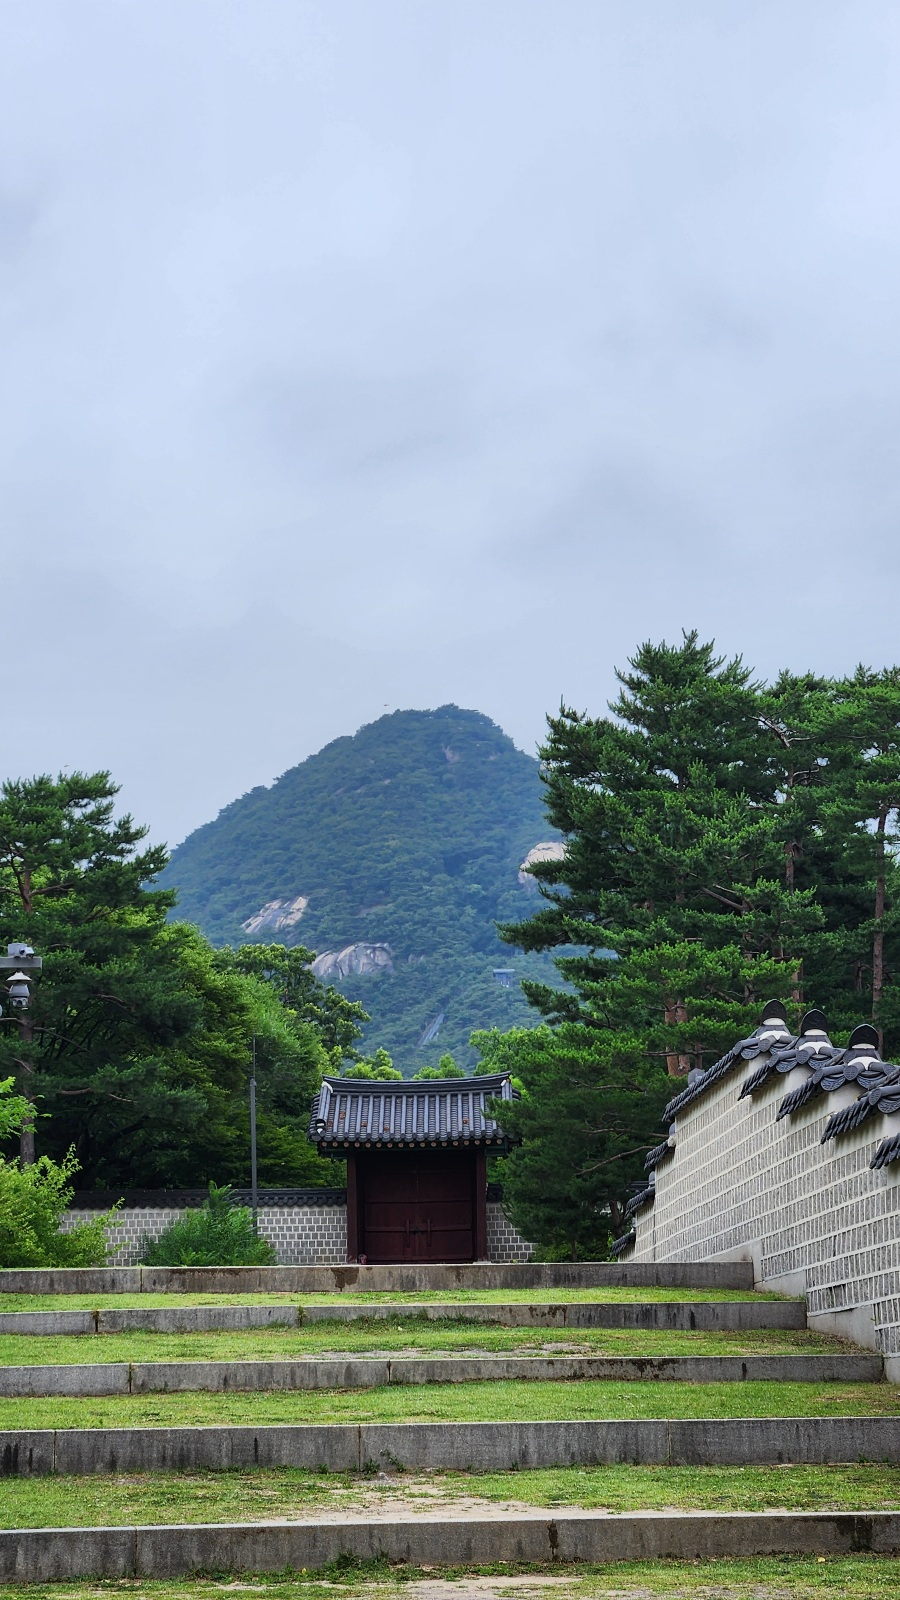
\includegraphics[height = 7cm]{20240630_143910}
        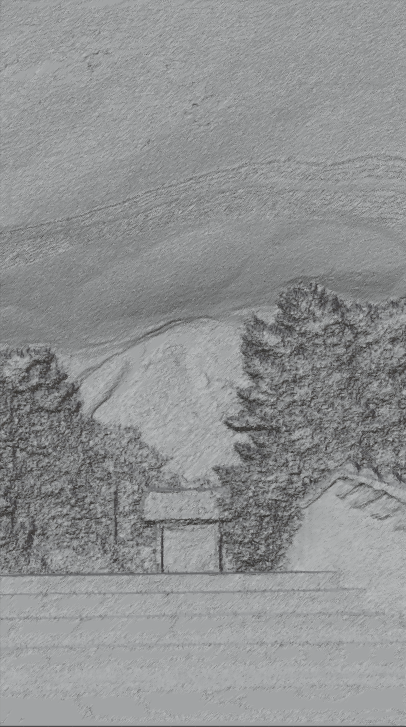
\includegraphics[height = 7cm]{20240630_143910_3d}
        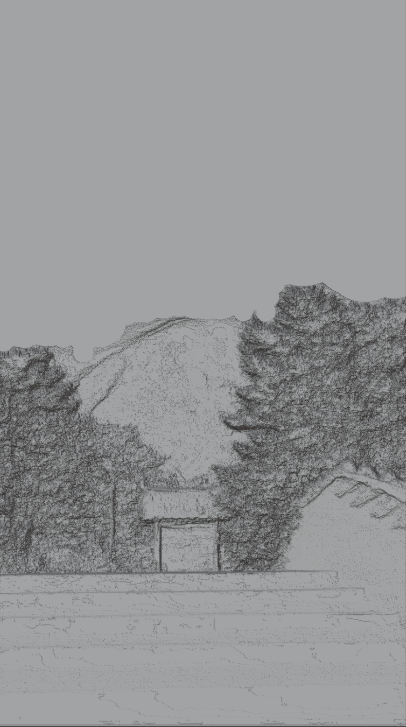
\includegraphics[height = 7cm]{20240630_143910_3dsky}
        \caption{Example of sky segmentation.}
        \label{skyseg}
    \end{center}
    \small
    In this image, we deem the sky irrelevant to the composition of the photo. The second image is a 3D reconstruction of the photo that takes the sky
    into consideration, while the third one has the sky removed \emph{manually} to give an idea of what this process would produce.
\end{figure}

In such cases, it can greatly reduce the number of vertices and faces, rendering the model more simple and easy to handle.

\paragraph{Relative depth} In this study, we have used relative depth maps. \emph{Relative depth} means that the pixel values indicate which points are closer or further away from the camera
without referencing real-world measurment, as opposed to \emph{Absolute depth} where each pixel value refers directly to a physical distance.
Because of this, our generated 3d models seem rather flat as compared to reality.

\begin{figure}[!ht]
    \begin{center}
        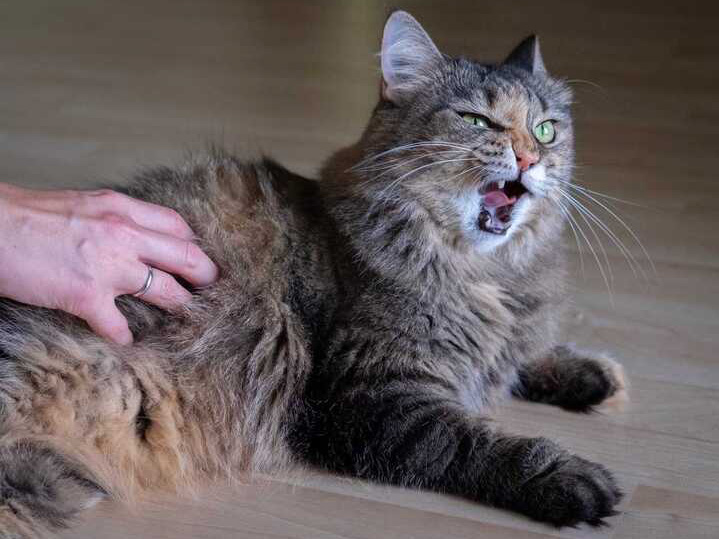
\includegraphics[height = 4cm]{example_5}
        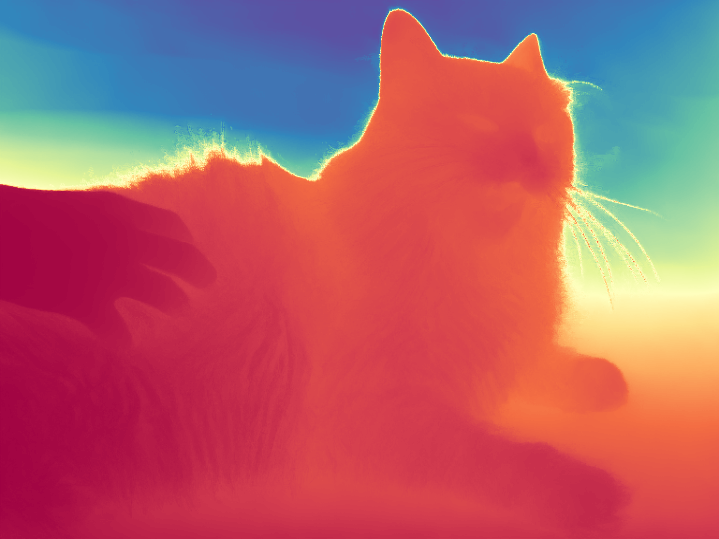
\includegraphics[height = 4cm]{example_5_pred_colored}
        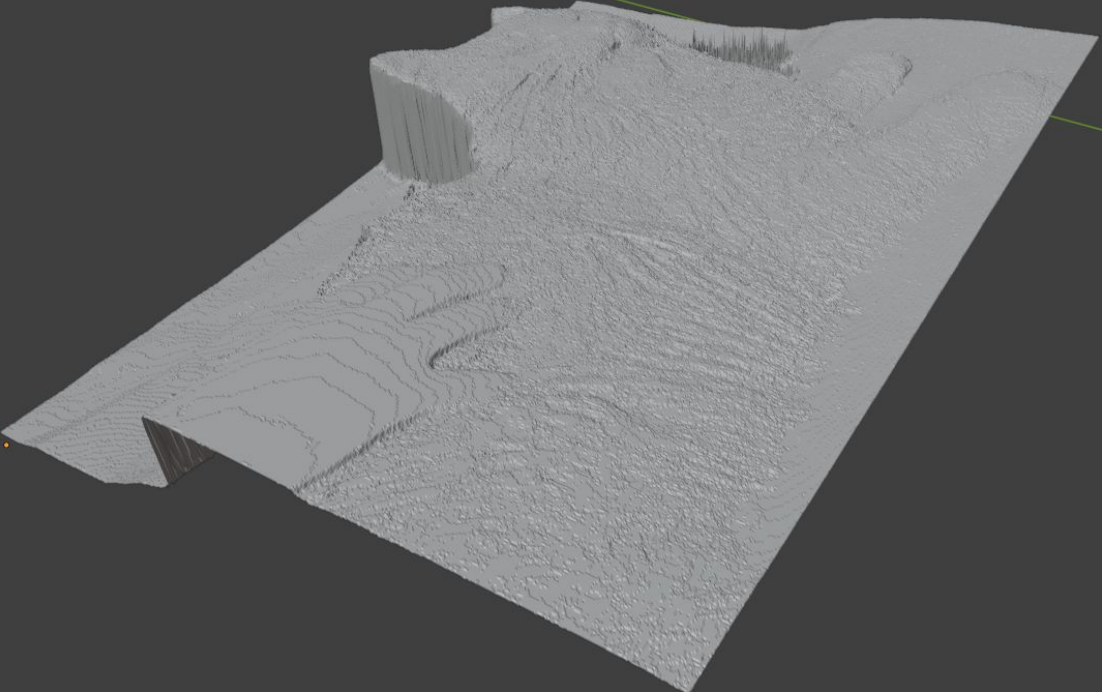
\includegraphics[height = 4cm]{relative_example_5_pred}
        \caption{Illustration of the relative depth interpretation issue.}
        \label{relative}
    \end{center}
\end{figure}

To address this issue, it can be interesting to use segmentation to identify and separate each individual object, and apply the depth estimation
on each of them. This would include fine-tuning the depth generation model, but it can theoretically be a solution to the relative depth problem.

\subsection{Evaluation method}

\paragraph{}
In our case, no research topic has been found that is relatively close to what we are studying, so evaluating the accuracy and usability of 3D
models in the absence of ground truth data is challenging, and we could not find the opportunity to test our method with practical tests. That
said, here are some methods we can consider to assess the quality of our generated 3D models before experimenting with visually impaired
individuals.

\paragraph{Qualitative Visual Inspection} We can have experts in computer vision or 3D modeling visually inspect the generated models
for consistency with the input images. They can evaluate the fidelity of the 3D shapes, contours, and surface details. We can also compare the
generated models with existing 3D models of similar objects available in public databases to assess visual similarity.

\paragraph{Synthetic Data Evaluation} One solution for evaluating our method would be synthetic data evaluation. Though it would be very time-consuming, we could
use a software to create synthetic 3D models with known properties and generate 2D images from these models. Afterwards, these images would be used as input to
the depth estimation and 3D modeling pipeline and the result would be compared to the synthetic ground truth.
Error metrics such as Mean Squared Error or Mean Absolute Error between the generated and synthetic ground truth model could prove useful.

\paragraph{Simulated Environment Testing} Integrating the 3D models into a virtual or augmented reality environment and have users with no visual impairment 
interact with them first can be an interesting approach. This can help in identifying any inconsistencies or issues with the models.

\newpage

%%%%%%%%%%%%%%%%%%%% CONCLUSION %%%%%%%%%%%%%%%%%%%%%%%%
\section{Conclusion}
\paragraph{}

In a world dominated by visual information, individuals with visual impairments face substantial challenges in understanding and engaging with their surroundings.
The inability to access and interpret visual cues creates a ``sensory gap", an inequality in information access due to sensory differences. This gap affects not
only those who are completely blind but also the broader community of 2.2 billion people worldwide with varying degrees of visual impairment. This study explores
methods to bridge this sensory gap, offering insights into how visually impaired individuals can perceive objects at a reduced scale, thereby enhancing their
interaction with the world.
The development of tactile photos using generative AI and 3D printing represents a significant step forward in bridging the sensory gap for individuals with
visual impairments. This thesis has explored the potential of integrating advanced technologies to create a more immersive, detailed, and inclusive tactile experience,
aiming to offer individuals with visual impairments a new way to engage with visual content.

The work conducted throughout this research demonstrates that current depth estimation models can effectively generate depth maps from 2D images, which can
then be transformed into 3D models suitable for tactile exploration. By focusing on the visible part of objects and emphasizing contours and shapes, the proposed
method allows for the creation of tactile photos.
\paragraph{}
The proposed pipeline is designed to be automated and user-friendly, enabling individuals with visual impairments to generate tactile photos without
requiring prior technical knowledge. This focus on simplicity and autonomy ensures that the technology can be easily integrated into educational
settings and everyday life, providing a valuable tool for learning and artistic expression. If it could be tested on the concerned individuals,
this research would contribute to the emphasis on usability and accessibility. 
\paragraph{}
However, the research also highlights several challenges and areas for future work. The current models, while effective in capturing object shapes and contours,
still face limitations in accurately representing surface geometry and finer details. Addressing these challenges will be crucial in improving the realism and
effectiveness of the tactile photos. The lack of ground truth 3D models also poses a challenge for the evaluation of the generated tactile models.
Moreover, the computational demands of generating high-resolution 3D models were significant, and attempts to simplify the models through post-processing
decimation introduced concerns about the tactile quality of the final output. Additionally, the reliance on relative depth
maps posed limitations, resulting in flatter-than-expected 3D representations. Future work could address these challenges by exploring sky segmentation 
techniques, object-specific depth estimation, and refining evaluation methods, potentially incorporating qualitative visual inspections and synthetic data
evaluations.

The implications of this research extend beyond the creation of tactile photos. The integration of AI and 3D printing has the potential to revolutionize the way
visual information is presented to individuals with visual impairments, offering new possibilities for education and accessibility. By continuing to refine
the proposed methods and exploring new applications, this technology could play a crucial role in fostering a more inclusive society where
visual content is accessible to all.
\paragraph{}
In conclusion, this thesis lays the groundwork for a promising approach to creating tactile photos that can enhance the lives of individuals with visual
impairments. While there are still challenges to overcome, the progress made in this research represents a significant step towards making visual content more
accessible and enjoyable for everyone. Continued exploration and innovation in this field will be essential to realizing the full potential of this technology
and its impact on accessibility and inclusion.

\end{spacing}
\newpage

%\bibliography{}

\section{Bibliography}

\paragraph{[WHO]}
\hypertarget{WHOtarget}{}
World Health Organisation, \textit{Blindness and visual impairment} \\
\href{https://www.who.int/news-room/fact-sheets/detail/blindness-and-visual-impairment}{https://www.who.int/news-room/fact-sheets/detail/blindness-and-vi}

\paragraph{[NM]}
\hypertarget{NMtarget}{}
News Medical Life Sciences, \textit{Types of visual impairment}
\href{https://www.news-medical.net/health/Types-of-visual-impairment.aspx}{https://www.news-medical.net/health/Types-of-visual-impairment.aspx}

\paragraph{[MBC22]}
\hypertarget{MBC22target}{}
Mukhiddinov, M.; Abdusalomov, A.B.; Cho, J. Automatic Fire Detection and Notification System Based on Improved YOLOv4 for the Blind and Visually Impaired. Sensors 2022, 22, 3307.
\href{https://doi.org/10.3390/s22093307}{https://doi.org/10.3390/s22093307}

\paragraph{[SeeAI]}
\hypertarget{SeeAItarget}{}
Microsoft, \textit{Seeing AI}
\href{https://www.microsoft.com/en-us/ai/seeing-ai}{https://www.microsoft.com/en-us/ai/seeing-ai}

\paragraph{[Ken93]}
\hypertarget{Ken93target}{}
Kennedy, J. M. (1993). Drawing \& the blind: Pictures to touch (1st ed.). New Haven, CT: Yale University Press.\\
\href{https://tspace.library.utoronto.ca/handle/1807/1021}{https://tspace.library.utoronto.ca/handle/1807/1021}

\paragraph{[LWX08]}
\hypertarget{LWXtarget}{}
J. Lu, K. W. M. Siu and P. Xu, ``A comparative study of tactile paving design standards in different countries," 2008 9th International Conference on\\
Computer-Aided Industrial Design and Conceptual Design, Beijing, China, 2008, pp. 753-758, doi: 10.1109/CAIDCD.2008.4730674.\\
\href{https://ieeexplore.ieee.org/abstract/document/4730674}{https://ieeexplore.ieee.org/abstract/document/4730674}

\paragraph{[LM08]}
\hypertarget{LM08target}{}
O.Lahav, D.Mioduser, ``Haptic-feedback support for cognitive mapping of unknown spaces by people who are blind", International Journal of Human-Computer Studies, Volume 66, Issue 1,
2008, Pages 23-35, ISSN 1071-5819,

\href{https://doi.org/10.1016/j.ijhcs.2007.08.001}{https://doi.org/10.1016/j.ijhcs.2007.08.001}

\paragraph{[GPM14]}
\hypertarget{GPM14target}{}
Ian J. Goodfellow, Jean Pouget-Abadie, Mehdi Mirza, Bing Xu, David Warde-Farley, Sherjil Ozair, Aaron Courville, Yoshua Bengio, ``Generative Adversarial Networks"
\href{https://arxiv.org/abs/1406.2661}{https://arxiv.org/abs/1406.2661}

\paragraph{[GMR18]}
\hypertarget{GMR18target}{}
Robert Geirhos, Carlos R. Medina Temme, Jonas Rauber, Heiko H. Schütt, Matthias Bethge, Felix A. Wichmannm ``Generalisation in humans and deep neural networks"
\href{https://arxiv.org/abs/1808.08750}{https://arxiv.org/abs/1808.08750}

\paragraph{[BKH14]}
\hypertarget{BKH14target}{}
Erin Buehler, Shaun K. Kane, and Amy Hurst. 2014. ``ABC and 3D: opportunities and obstacles to 3D printing in special education environments".
In Proceedings of the 16th international ACM SIGACCESS conference on Computers \& accessibility (ASSETS '14). Association for Computing Machinery, New York, NY, USA, 107–114.
\href{https://doi.org/10.1145/2661334.2661365}{https://doi.org/10.1145/2661334.2661365}

\paragraph{[GP18]}
\hypertarget{GP18target}{}
N. Giudice, H. P. Palani, J. Gorlewicz, J. Tennison (2018). The Graphical Access Challenge for People with Visual Impairments: Positions and Pathways Forward.
\href{https://www.researchgate.net/publication/330940759_The_Graphical_Access_Challenge_for_People_with_Visual_Impairments_Positions_and_Pathways_Forward}{10.5772/intechopen.82289.}

\paragraph{[PCS24]}
\hypertarget{PCS24target}{}
Eduardo Puerta, Tarik Crnovrsanin, Laura South, and Cody Dunne. 2024. The Effect of Orientation on the Readability and Comfort of 3D-Printed Braille.
In Proceedings of the CHI Conference on Human Factors in Computing Systems (CHI '24). Association for Computing Machinery, New York, NY, USA, Article 346, 1–15.
\href{ https://doi.org/10.1145/3613904.3642719}{ https://doi.org/10.1145/3613904.3642719}

\paragraph{[RLH20]}
\hypertarget{RLH20target}{}
R. Ranftl, K. Lasinger, D. Hafner, K. Schindler and V. Koltun, ``Towards Robust Monocular Depth Estimation: Mixing Datasets for Zero-Shot Cross-Dataset Transfer,"
in IEEE Transactions on Pattern Analysis and Machine Intelligence, vol. 44, no. 3, pp. 1623-1637, 1 March 2022
\href{https://arxiv.org/pdf/1907.01341v3}{https://arxiv.org/pdf/1907.01341v3}


\paragraph{[Hel00]}
\hypertarget{Hel00target}{}
Heller, Morton A. (ed.), Touch, Representation, and Blindness, Debates in Psychology (Oxford, 2000; online edn, Oxford Academic, 22 Mar. 2012),\\
\href{https://academic.oup.com/book/10831}{https://academic.oup.com/book/10831}, accessed 31 July 2024.


\paragraph{[KOH24]}
\hypertarget{KOH24target}{}
Bingxin Ke and Anton Obukhov and Shengyu Huang and Nando Metzger and Rodrigo Caye Daudt and Konrad Schindler,
Repurposing Diffusion-Based Image Generators for Monocular Depth Estimation, 2024\\
\href{https://arxiv.org/abs/2312.02145}{https://arxiv.org/abs/2312.02145}


\paragraph{[EPF14]}
\hypertarget{EPF14target}{}
David Eigen and Christian Puhrsch and Rob Fergus, Depth Map Prediction from a Single Image using a Multi-Scale Deep Network 2014\\
\href{https://arxiv.org/abs/1406.2283}{https://arxiv.org/abs/1406.2283}

\paragraph{[RNR12]}
\hypertarget{RNR12target}{}
Andreas Reichinger, Moritz Neumuller, Florian Rist, Stefan Maierhofer, and Werner Purgathofer. 2012.
Computer-Aided design of tactile models: taxonomy and case studies.In Proceedings of the 13th international conference on Computers Helping People with Special Needs - Vol. Part II. Springer-Verlag, Berlin, Heidelberg
\href{https://link.springer.com/chapter/10.1007/978-3-642-31534-3\_73}{https://link.springer.com/chapter/10.1007/978-3-642-31534-3\_73}

\paragraph{[LLS23]}
\hypertarget{LLS23target}{}
Liu, Zhong and Li, Ran and Shao, Shuwei and Wu, Xingming and Chen, Weihai. 2023.
Self-Supervised Monocular Depth Estimation With Self-Reference Distillation and Disparity Offset Refinement, Vol. 33. IEEE Transactions on Circuits and Systems for Video Technology
\href{https://arxiv.org/pdf/2302.09789}{https://arxiv.org/pdf/2302.09789}


\newpage


\appendix
\addcontentsline{toc}{section}{\appendixname}


\begin{figure}[!ht]
    \begin{center}
        \includegraphics[height = 3.3cm]{fe414_0000722049_1}
        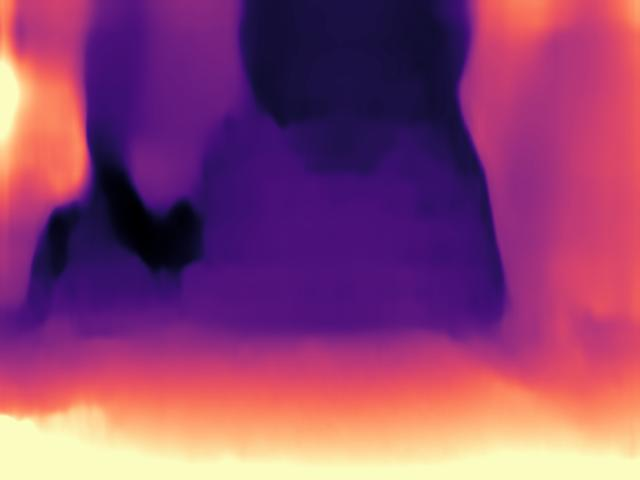
\includegraphics[height = 3.3cm]{fe414_0000722049_1_disp}
        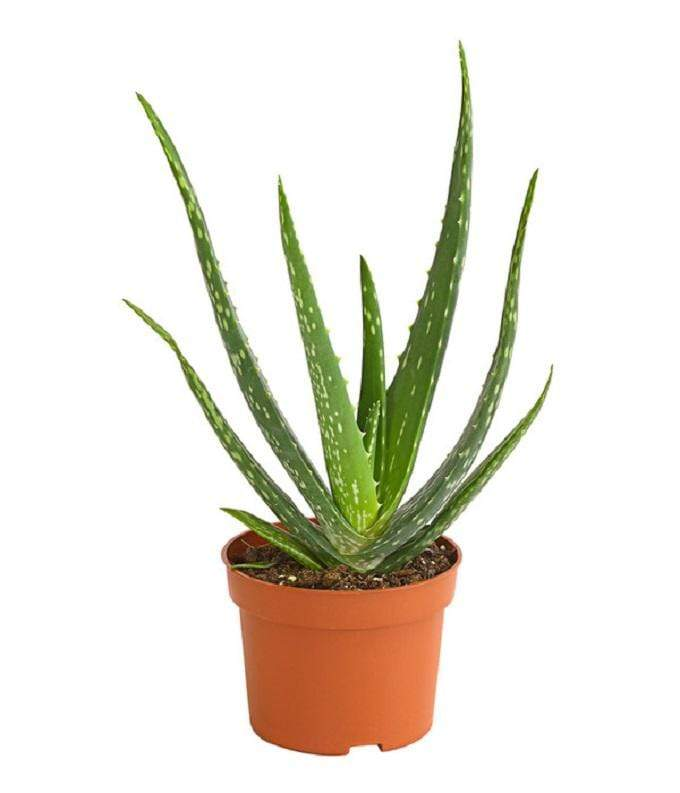
\includegraphics[height = 3.3cm]{jardins-du-senegal-aloe-vera-28830638178417_1200x1200}
        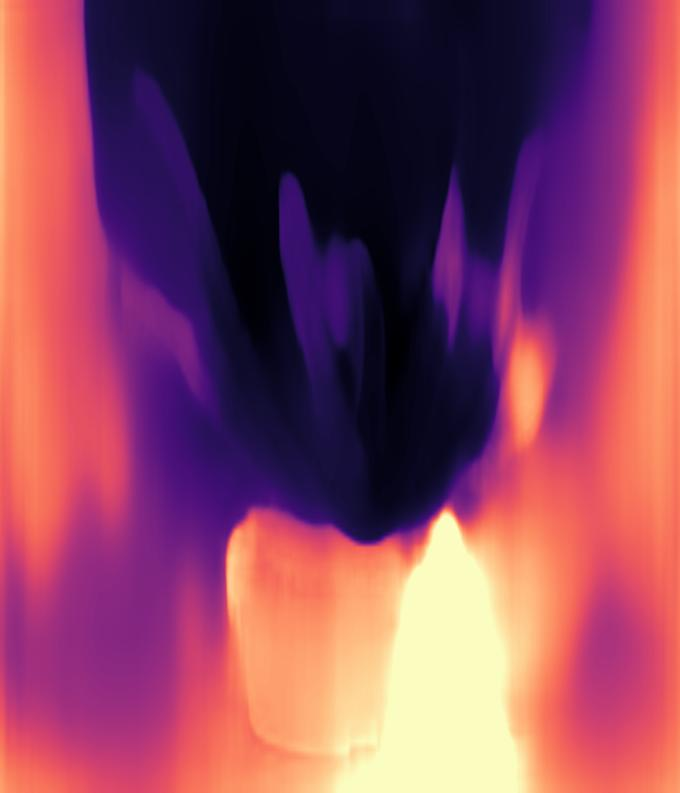
\includegraphics[height = 3.3cm]{jardins-du-senegal-aloe-vera-28830638178417_1200x1200_disp}

        \includegraphics[height = 3.5cm]{Rue_Blanche_-_Paris_IX_(FR75)_-_2021-06-28_-_1}
        \includegraphics[height = 3.5cm]{RueBlancheStero1024}
        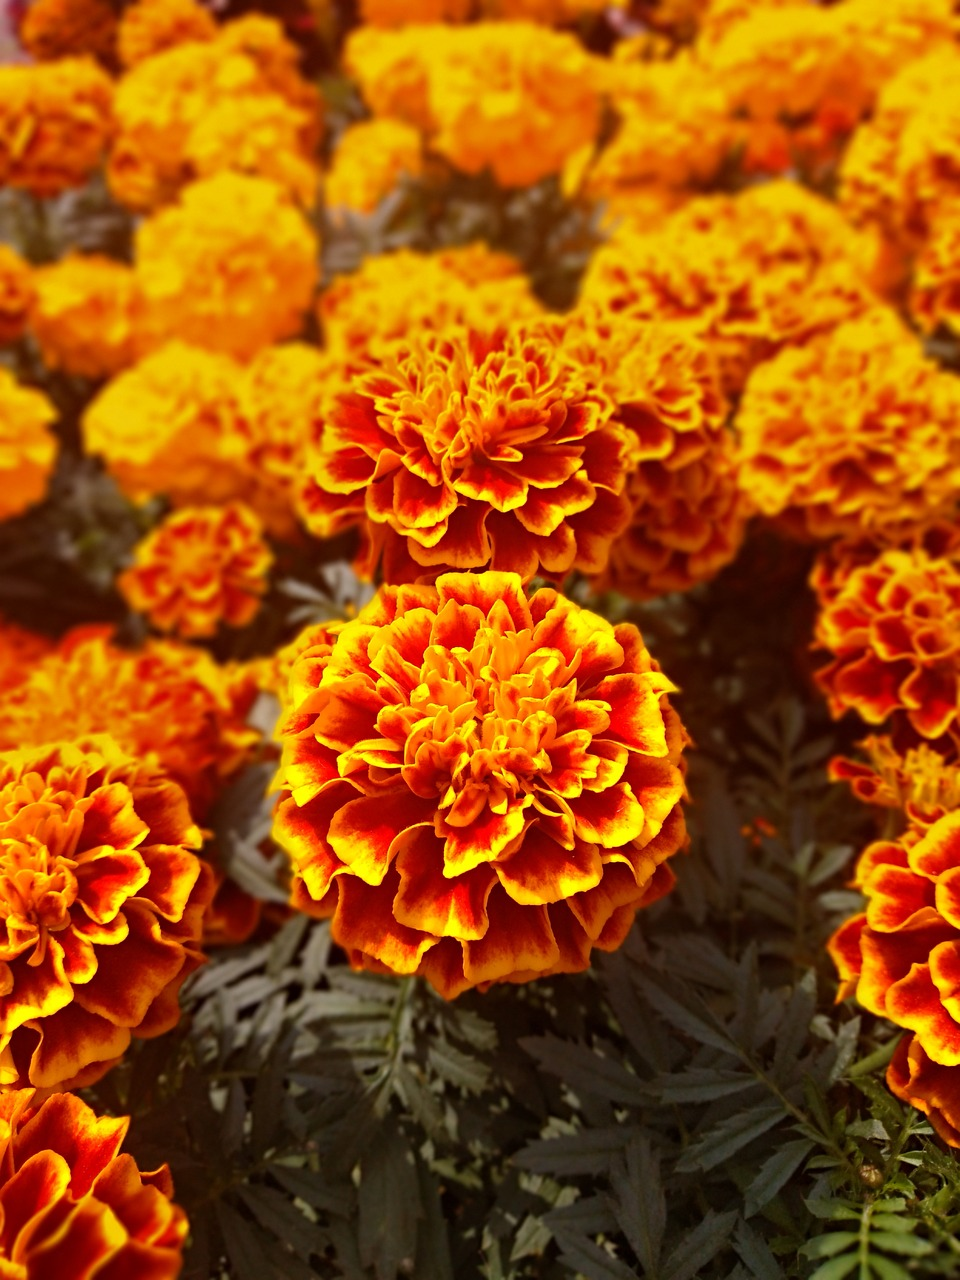
\includegraphics[height = 3.5cm]{example_0}
        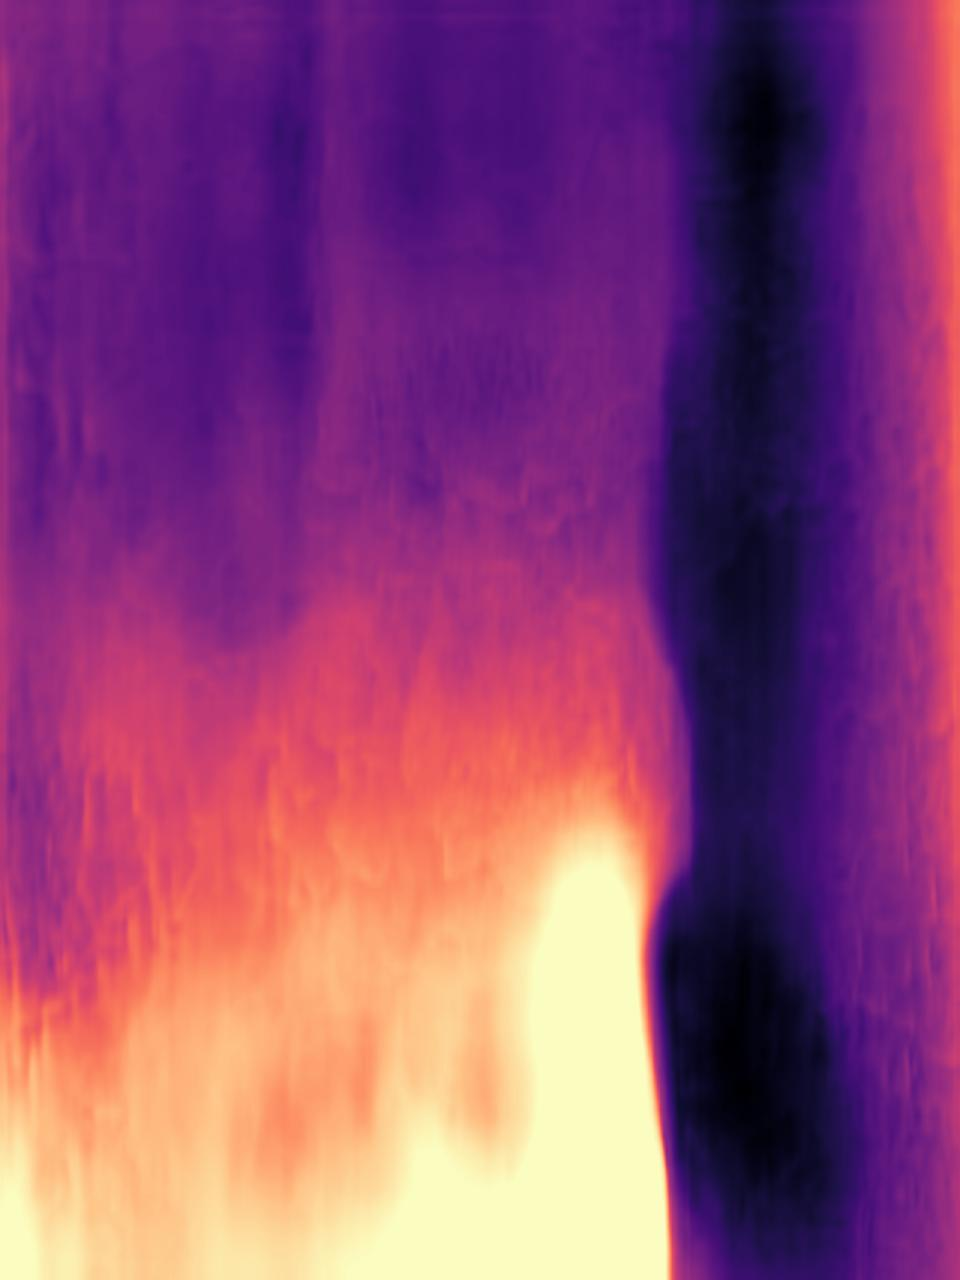
\includegraphics[height = 3.5cm]{example_0_disp}
        \caption{Examples of failed depth maps generated by SRD.}
        \label{appSRD}
    \end{center}
\end{figure}
\vspace{2 cm}
\begin{figure}[!ht]
    \begin{center}
        \includegraphics[height = 3.2cm]{himejicastle_event_2}
        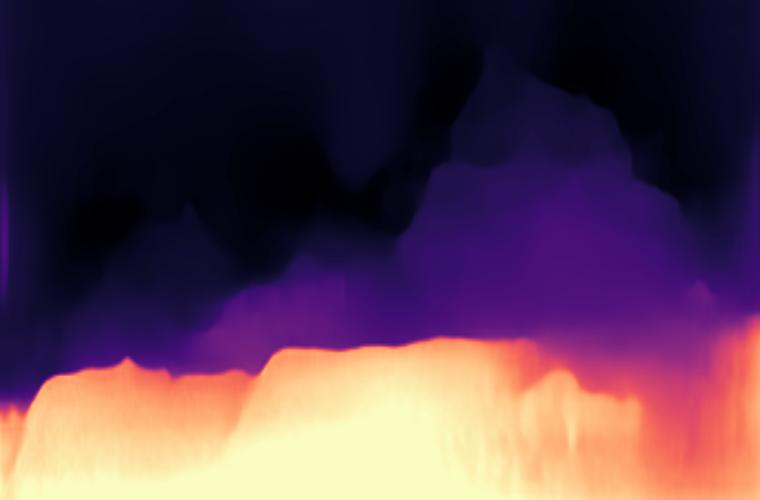
\includegraphics[height = 3.2cm]{himejicastle_event_2_disp}
        \includegraphics[height = 3.2cm]{himejicastle_event_2_pred_colored}\\
        \includegraphics[height = 1.8cm]{test_image}
        \includegraphics[height = 1.8cm]{test_image_disp}
        \includegraphics[height = 1.8cm]{test_image_pred_colored}

        \caption{Comparing usable SRD and Marigold results.}
        \label{compSRDMRG}
    \end{center}
\end{figure}

\begin{figure}[!ht]
    \centering
    \begin{minipage}{0.22\textwidth}
        \includegraphics[width=\textwidth]{example_0}
        \includegraphics[width=\textwidth]{example_2}
        \includegraphics[width=\textwidth]{example_4}
        \includegraphics[width=\textwidth]{example_6}
    \end{minipage}
    \begin{minipage}{0.22\textwidth}
        \includegraphics[width=\textwidth]{example_0_pred_colored}
        \includegraphics[width=\textwidth]{example_2_pred_colored}
        \includegraphics[width=\textwidth]{example_4_pred_colored}
        \includegraphics[width=\textwidth]{example_6_pred_colored}
    \end{minipage}
    \begin{minipage}{0.22\textwidth}
        \includegraphics[width=\textwidth]{example_1}
        \includegraphics[width=\textwidth]{example_3}
        \includegraphics[width=\textwidth]{example_5}
        \includegraphics[width=\textwidth]{example_7}
    \end{minipage}
    \begin{minipage}{0.22\textwidth}
        \includegraphics[width=\textwidth]{example_1_pred_colored}
        \includegraphics[width=\textwidth]{example_3_pred_colored}
        \includegraphics[width=\textwidth]{example_5_pred_colored}
        \includegraphics[width=\textwidth]{example_7_pred_colored}
    \end{minipage}
    \caption{Non exhaustive list of RGB depth maps generated by Marigold.}
    \label{MRGfull}
\end{figure}

\begin{figure}[!ht]
    \begin{center}
        \includegraphics[height = 6.5cm]{20240630_143910_3dsky}
        \includegraphics[height = 6.5cm]{example_6.png}
        \includegraphics[height = 6.5cm]{example_0_pred_colored_3d}
        \includegraphics[height = 4.7cm]{himejicastle_event_2_3d}
        \includegraphics[height = 4.7cm]{example_5_3d}
        \includegraphics[height = 5cm]{test_image_pred_colored3d}

        \caption{Non exhaustive list of 3D models produced using depth maps generated by Marigold.}
        \label{3dmod}
    \end{center}
\end{figure}

% \hline
% $680 \times 793$ & 539,240 & 1,075,536 & 220.96 seconds\\ 

\end{document}
